
\documentclass[a4paper,UKenglish,cleveref, autoref, thm-restate, anonymous]{lipics-v2021}
%This is a template for producing LIPIcs articles.
%See lipics-v2021-authors-guidelines.pdf for further information.
%for A4 paper format use option "a4paper", for US-letter use option "letterpaper"
%for british hyphenation rules use option "UKenglish", for american hyphenation rules use option "USenglish"
%for section-numbered lemmas etc., use "numberwithinsect"
%for enabling cleveref support, use "cleveref"
%for enabling autoref support, use "autoref"
%for anonymousing the authors (e.g. for double-blind review), add "anonymous"
%for enabling thm-restate support, use "thm-restate"
%for enabling a two-column layout for the author/affilation part (only applicable for > 6 authors), use "authorcolumns"
%for producing a PDF according the PDF/A standard, add "pdfa"

%\pdfoutput=1 %uncomment to ensure pdflatex processing (mandatatory e.g. to submit to arXiv)
%\hideLIPIcs  %uncomment to remove references to LIPIcs series (logo, DOI, ...), e.g. when preparing a pre-final version to be uploaded to arXiv or another public repository

%\graphicspath{{./graphics/}}%helpful if your graphic files are in another directory


%%%% Ours %%%%
\usepackage{algorithm}
\usepackage{algorithmic}
\renewcommand{\algorithmiccomment}[1]{\hfill  {\small  \tt \# #1}}

\usepackage{amsmath}
\usepackage{dsfont}
\usepackage{mathbbol}

\newcommand{\pred}{\texttt{pred}}
\newcommand{\vect}[1]{\ensuremath{\mathbf{#1}}}
\newcommand{\one}{\ensuremath{\mathds{1}}}
%%%%%%%%%%%%%%


\bibliographystyle{plainurl}% the mandatory bibstyle

\title{Online Primal-Dual Algorithm with Predictions\\for Non-Linear Covering Problems} %TODO Please add

%%\titlerunning{Dummy short title} %TODO optional, please use if title is longer than one line
%\author{Kevi Enik\H{o}}{Université Grenoble Alpes, France}{eniko.kevi@univ-grenoble-alpes.fr}{}{}%TODO mandatory, please use full name; only 1 author per \author macro; first two parameters are mandatory, other parameters can be empty. Please provide at least the name of the affiliation and the country. The full address is optional. Use additional curly braces to indicate the correct name splitting when the last name consists of multiple name parts.
%
%\author{Nguyen Kim Thang}{Université Grenoble Alpes, France}{kim-thang.nguyen@univ-grenoble-alpes.fr}{}{}
%\authorrunning{Kevi Enik\H{o} and Nguyen Kim Thang} %TODO mandatory. First: Use abbreviated first/middle names. Second (only in severe cases): Use first author plus 'et al.'

\Copyright{Kevi Enik\H{o} and Nguyen Kim Thang} %TODO mandatory, please use full first names. LIPIcs license is "CC-BY";  http://creativecommons.org/licenses/by/3.0/

\ccsdesc[500]{{Theory of computation~Online learning algorithms}}
%TODO mandatory: Please choose ACM 2012 classifications from https://dl.acm.org/ccs/ccs_flat.cfm

\keywords{non-linear objective, learning-augmented algorithm, primal-dual algorithm, covering problems, predictions, online algorithm with advice} %TODO mandatory; please add comma-separated list of keywords

%\category{} %optional, e.g. invited paper

%\relatedversion{} %optional, e.g. full version hosted on arXiv, HAL, or other respository/website
%\relatedversiondetails[linktext={opt. text shown instead of the URL}, cite=DBLP:books/mk/GrayR93]{Classification (e.g. Full Version, Extended Version, Previous Version}{URL to related version} %linktext and cite are optional

%\supplement{}%optional, e.g. related research data, source code, ... hosted on a repository like zenodo, figshare, GitHub, ...
%\supplementdetails[linktext={opt. text shown instead of the URL}, cite=DBLP:books/mk/GrayR93, subcategory={Description, Subcategory}, swhid={Software Heritage Identifier}]{General Classification (e.g. Software, Dataset, Model, ...)}{URL to related version} %linktext, cite, and subcategory are optional

%\funding{(Optional) general funding statement \dots}%optional, to capture a funding statement, which applies to all authors. Please enter author specific funding statements as fifth argument of the \author macro.

%\acknowledgements{I want to thank \dots}%optional

%\nolinenumbers %uncomment to disable line numbering



%Editor-only macros:: begin (do not touch as author)%%%%%%%%%%%%%%%%%%%%%%%%%%%%%%%%%%
\EventEditors{John Q. Open and Joan R. Access}
\EventNoEds{2}
\EventLongTitle{42nd Conference on Very Important Topics (CVIT 2016)}
\EventShortTitle{CVIT 2016}
\EventAcronym{CVIT}
\EventYear{2016}
\EventDate{December 24--27, 2016}
\EventLocation{Little Whinging, United Kingdom}
\EventLogo{}
\SeriesVolume{42}
\ArticleNo{23}
%%%%%%%%%%%%%%%%%%%%%%%%%%%%%%%%%%%%%%%%%%%%%%%%%%%%%%

\begin{document}

\maketitle

\begin{abstract}
    Auctions with divisible resources represent various practically relevant problems, such as network bandwidth allocation and food aid distribution. In each of these settings, the desire to receive (or the need of) a resource is represented by bids. The proportional allocation mechanism assigns a fraction of the resource to each bidder in proportion to the bid across all the bids. Despite the importance of these type of auctions, the efficiency of proportional allocations is still not completely understood. In recent years, \cite{Tardos2013} proved a lower bound of $26.8\%$ for the Price of Anarchy (PoA) considering social welfare, and \cite{Caragiannis2014} improved their analysis to $50\%$ both for social and effective welfares. This paper follows a different perspective on the analysis of this problem, which relies on the primal-dual method (first introduced in this setting by \cite{Thang2017}). We prove that the Price of Anarchy (PoA) bound considering the effective welfare of proportional allocation over coarse-correlated and Bayes-Nash equilibria in the complete information setting for a single item is $50\%$, and this result is \emph{tight}.
\end{abstract}

%!TEX root = ./main.tex

\section{Introduction}

% Introduction and motivation for our problem
% main objective: compare the best combination of experts.
% So for in the literature, always compare to the best expert (ex., regret)

The domain of algorithms with predictions \cite{MitzenmacherVassilvitskii20:Beyond-the-Worst-Case}  (or learning-augmented algorithms) emerged recently and grew immensely at the intersection of (discrete) algorithm design and machine learning (ML).
Combining ML techniques with traditional algorithm design methods enables online algorithms to benefit from predictions that can infer future information from patterns in past data. Online algorithms with predictions can obtain performance guarantees beyond the worst-case analysis and provide fine-tuned solutions to various problems. In the literature, many significant problems have new learning-augmented results, for example, scheduling \cite{LattanziLavastida20:Online-scheduling,Mitzenmacher20:Scheduling-with}, caching (paging) \cite{LykourisVassilvtiskii18:Competitive-caching,Rohatgi20:Near-optimal-bounds,AntoniadisCoester20:Online-metric}, ski rental \cite{GollapudiPanigrahi19:Online-algorithms,KumarPurohit18:Improving-online,AngelopoulosDurr20:Online-Computation}, counting sketches \cite{HsuIndyk19:Learning-Based-Frequency}, bloom filters \cite{KraskaBeutel18:The-case-for-learned,Mitzenmacher18:A-model-for-learned}, and metrical task systems \cite{AntoniosEtAll23:mixing-predictions-metric-algorithms}.

Even though predictions provide a glimpse of the future, there is no mathematical guarantee for their accuracy. Adjusting the algorithm's trust in the predictions is a significant challenge since online algorithms must make irrevocable decisions at each time step. Ideally, if the predictions are accurate, the algorithm should perform well compared to the offline setting. In contrast, if the predictions are misleading, the algorithm should maintain a competitive solution, similar to the online setting where no predictive information is available. In other words, online algorithms with predictions are expected to bring the best of both worlds: mathematical performance guarantees of classical algorithms and good future prediction capabilities of machine learning methods.

Predictions can come from multiple sources (for example: heuristics, oracles, and randomized methods), but we ignore their nature and call all of them \emph{experts}.  An algorithm's consistency with the experts' suggestions is typically measured by comparing the algorithm's result with the solution of the \emph{best} expert. A representative example is the popular notion of regret in online learning, which fueled the development of many powerful algorithms and techniques.

A natural research question is whether it is possible to design competitive algorithms with mathematical performance guarantees with a stronger benchmark than the best expert. Comparing an algorithm with a stronger benchmark could provide deeper insights into the learning process and give better ways of exploiting the experts' predictions.

Taking a broader view, we can study whether combining predictions of several experts is similar to combining multiple online algorithms and whether we can expect to achieve better solutions with the combination. Assuming that we do not know in advance which of the given algorithms would perform best on the upcoming requests, can we combine the algorithms in some generic way to obtain a competitive online strategy? This has been a long-standing question in the community of online algorithms \cite{AzarBroder93:On-line-Choice,BlumBurch00:On-line-Learning}. To find an answer, it is a crucial to understand to what extent such an online strategy can benefit from the input of multiple algorithms and what is a suitable benchmark to evaluate its performance.

While in a completely general setting such an online strategy and a corresponding benchmark may not exist, in this paper we propose
two algorithms for online linear and convex problems with covering constraints that are competitive with the new benchmark (informally the \emph{best linear combination} of the experts). Therefore, our paper partially addresses the question we raised in the previous paragraph.

\subsection{Model and Problem}

\paragraph{Covering problem with experts.}
In the linear problem setting, we have $n$ resources and each resource $i$ has a cost per unit $c_{i}$ that we know in advance ($1 \leq i \leq n$).
Let $x_{i}$ be a non-negative variable representing the amount chosen from resource $i$.
The total cost of a solution $(x_{i})_{i=1}^{n}$ is $\sum_{i=1}^{n} c_{i} x_{i}$.
The problem includes $K$ experts and the problem's covering-type constraints are revealed online one-by-one.
At each time $t \geq 1$, we receive a covering constraint $\sum_{i=1}^{n} a_{i}^{t} x_{i} \geq 1$ (where $a_{i}^{t} \geq 0$) and each expert $k$ (where $1 \leq k \leq K$) provides
a solution $(s_{i,k}^{t})_{i=1}^{n}$. Our algorithm can observe the experts' solutions and afterwards it must update its own solution (denoted as $(x_{i}^{t})_{i=1}^{n}$)
to satisfy the new constraint, while maintaining the satisfaction of the previous ones. This algorithm must update its solution in the sense of online algorithms, so it cannot modify the previously made decisions. Formally, $x_{i}^{t} \geq x_{i}^{t-1} ~\forall\ i, t$.
Our goal is to design an algorithm that minimizes $\sum_{i=1}^{n} c_{i} x_{i}^{T}$ subject to
all online covering constraints $t$, where $1 \leq t \leq T$. The value $T$ is the last time a constraint is released, and it is not known by the algorithm.

The convex problem setting is analogous to the linear one, since we consider convex problems with linear constraints. The only difference compared to the previous paragraph is the total cost of the solution $(x_{i})_{i=1}^{n}$, which becomes $f(x)$, where $f$ is a convex function.

\paragraph{Experts.} \label{subsec:experts} In our model, the experts' predictions are also online solutions. In other words, the experts' solutions
fulfill the following properties:
\begin{enumerate}
	\item for every expert $k$ and for every time $t$ the solution $(s_{i,k}^{t})_{i=1}^{n}$ is feasible, therefore, every constraint $t'$ where $1 \leq t' \leq t$ is satisfied;
	\item for every expert $k$ and for every time $t$ and for every resource $i$, the previous expert solutions are irrevocable, therefore $s_{i,k}^{t} \geq s_{i,k}^{t'}$ for all $t' \leq t$.
\end{enumerate}
These properties can be verified online. If some experts do not satisfy them, we simply ignore those experts both in the decision-making and in the benchmark.
A crucial remark: we do \emph{not} assume that the experts' solutions are tight at each constraint $t$, requiring $\sum_{i=1}^{n} a_{i}^{t} s_{i,k}^{t} = 1 ~ \forall t, k$ to hold.
This assumption is unrealistic and cannot be maintained in an online manner (see the discussion in Appendix~\ref{appix-tight-solutions}).
Besides, assuming tight constraint satisfaction would simplify the problem, while intuitively,
the difficulty of designing competitive algorithms comes from the lack of obvious ways to distinguish
good expert solutions from (probably many) non-efficient/misleading ones.

\paragraph{Benchmark.}
We consider a dynamic benchmark that captures the \emph{best linear combination} of all experts' solutions \emph{over time}.
Informally, at any online time step, the benchmark can take a linear combination of the experts' solutions.
The linear combination can be changed over time, and it can be different from previous combinations.
However, the benchmark's decisions are also online, so it cannot decrease the value of the decision variables ($x_{i}$).
We refer to our benchmark with the name \texttt{LIN-COMB} from now on.

The \texttt{LIN-COMB} benchmark's formal description is visible on \cref{fig:benchmark}.
Let $w_{k}^{t} \geq 0$ be the weight assigned by the \texttt{LIN-COMB} benchmark to expert $k$ (where $1 \leq k \leq K$) at time~$t$.
Since we consider a linear combination, the constraint $ \sum_{k=1}^{K} w_{k}^{t} = 1$ must hold.
%In the linear program, we consider the relaxed version of this constraint, where $\sum_{k=1}^{K} w_{k}^{t} \geq 1$.
The solution of \texttt{LIN-COMB} at time $t$ is ideally $x_{i}^{t} = \sum_{k=1}^{K} w_{k}^{t} s_{i,k}^{t}$,
however, $x_{i}^{t}$ must be larger than $x_{i}^{t-1}$.
Therefore, we set $x_{i}^{t} = \max\bigl\{\sum_{k=1}^{K} w_{k}^{t} s_{i,k}^{t},\ x_{i}^{t-1}\bigr\}$.
In other words, given the chosen weights, if  $\sum_{k=1}^{K} w_{k}^{t} s_{i,k}^{t} < x_{i}^{t-1}$ then $x_{i}^{t} \gets x_{i}^{t-1}$,
otherwise $x_{i}^{t} \gets \sum_{k=1}^{K} w_{k}^{t} s_{i,k}^{t}$.

\begin{figure}[ht]
	\begin{mdframed}
	%	\begin{spacing}{0.1}
		\begin{align*}
			\text{Linear objective:} && \min \sum_{i=1}^{n} c_{i} x_{i}^{T} &= \min \sum_{i=1}^{n} c_{i} \sum_{t=1}^{T}\bigl( x_{i}^{t} - x_{i}^{t-1}\bigr)\\
			\text{Convex objective:} && \min f(x^{T}) &\\
	%	\end{align*}
	%	subject to
	%	\end{spacing}
	%	\begin{align*}
		&& & \\
		\text{Subject to (in both cases):} &&
			\sum_{k=1}^{K} w_{k}^{t} &= 1  && \forall\ t \\
			%
			&& x_{i}^{t} &\geq \sum_{k=1}^{K} w_{k}^{t} s_{i,k}^{t} && \forall\ i, t\\
			%
			&& x_{i}^{t} &\geq x_{i}^{t-1} && \forall\ i, t\\
			%
			&& w_{k}^{t} &\geq 0  && \forall\ t, k
		\end{align*}
		where $1 \leq t \leq T$, $1 \leq i \leq n$, and $f$ is convex.
		\vspace{5pt}
	\end{mdframed}
	\caption{Formulation of the \texttt{LIN-COMB} benchmark for both the linear and convex problems}
	\label{fig:benchmark}
	\end{figure}

Since every expert's solution is feasible by our assumptions, at each time $t$ and for all resource $i$ (where $1 \leq i \leq n$),
the constructed solution $x_{i}^{t} \geq \sum_{k=1}^{K} w_{k}^{t} s_{i,k}^{t}$ constitutes a feasible solution to the covering constraints of the original covering problem.
Formally, for every constraint $t'$ with $t' \leq t$,
%
\begin{align*}
\sum_{i=1}^{n} a_{i}^{t'} x_{i}^{t} \geq
%
\sum_{i=1}^{n} a_{i}^{t'} \biggl( \sum_{k=1}^{K} w_{k}^{t} s_{i,k}^{t} \biggr)
%
	= \sum_{k=1}^{K} w_{k}^{t}  \biggl( \sum_{i=1}^{n} a_{i}^{t'} s_{i,k}^{t} \biggr)
%
	\geq \sum_{k=1}^{K} w_{k}^{t} \geq 1
\end{align*}
%
where the second inequality holds due to the feasibility of the experts' solutions.
%
%Let $y_{i}^{t}$ be a variable representing the increase of $x_{i}^{t}$ compared to $x_{i}^{t-1}$. The benchmark is as follows.
%%
%\begin{align*}
%    && \min \sum_{t = 1}^{T} \sum_{i=1}^{n} & c_i y_i^t \\
%%
%    (\alpha^{t}) \qquad && \sum_{k=1}^{K} w_{k}^{t} & \geq 1  & \forall\ 1 \leq t \leq T,\ 1 \leq i \leq n \\
%%
%    (\beta_{i}^{t}) \qquad && \sum_{k=1}^{K} \left(w_{k}^{t} s_{i,k}^{t} - w_{k}^{t-1} s_{i,k}^{t-1} \right) &\leq y_i^t  &\forall\ 1 \leq t \leq T,\ 1 \leq i \leq n\\
%%
%    && w_{k}^{t},\ y_{i}^{t} & \ge 0 & \forall\ 1 \leq t \leq T,\ 1 \leq i \leq n,\ 1 \leq k \leq K
%\end{align*}
%
We highlight that the best-expert benchmark is included in \texttt{LIN-COMB}. We get the solution of this benchmark by setting $w^{t}_{k^{*}} = 1$ for all $t$, where $1 \leq t \leq T$, and $w^{t}_{k} = 0$ for all $k \neq k^{*}$,
where $k^{*}$ is the best expert (so $x_{i}^{t} = s_{i,k^{*}}^{t}$ for all $i$ and $t$).

\subsection{Our approach and contribution}

\paragraph{Approach.} We use the primal-dual approach to design competitive algorithms with the new \texttt{LIN-COMB} benchmark. First, we relax the linear program formulation of \texttt{LIN-COMB}, which serves as a lower bound. Then, we take the dual of the relaxation, which is a lower bound on the relaxation. Therefore, following the chain of lower bounds, the dual problem is a lower bound on the \texttt{LIN-COMB} benchmark. The formulations of the relaxation and its dual is detailed in \cref{sec:covering} for linear problems and in \cref{sec:convex} for convex problems.

Both of our proposed algorithms set the decision variables at every time step based on the solution of an internal convex program. Our approach is inspired by the
convex regularization method of \cite{BuchbinderChen14:Competitive-Analysis}, where the objective of the convex program is a shifted entropy function.
These functions have been widely used, in particular in the recent breakthrough related to $k$-server \cite{BubeckCohen18:K-server-via-multiscale,BuchbinderGupta19:k-servers-with}
and metrical task system problems \cite{BubeckCohen21:Metrical-task},
in which the entropy functions are shifted by constant parameters.

\paragraph{Novelty.} A novel point in our approach is that the entropy function is shifted by the average of the experts' solutions.
Moreover, regarding the constraints of the convex program, instead of using the experts' solutions directly,
we define auxiliary solutions that guarantee tight constraint satisfaction. We only use these tight solutions in the constraints and they play a crucial role in the proofs.

\paragraph{Results.} Let $\rho$ be the maximum ratio between the experts' solutions on the resources. Formally,
%We define the following parameter to establish the competitive ratio of our algorithm.
\[
	\rho := \max_{i} \max_{t',t''} \biggl\{\frac{\sum_{k=1}^{K} s_{i,k}^{t'}}{\sum_{k=1}^{K} s_{i,k}^{t''}} \biggr\}  \textnormal{ s.t. } \sum_{k=1}^{K} s_{i,k}^{t''} > 0.
\]
Informally, $\rho$ represents the discrepancy across the experts' predictions.
Our main result consists of two algorithms. The first one (which provides solutions for online linear covering) has an objective cost at most $O(\ln(K\rho))$ times the cost of the \texttt{LIN-COMB} benchmark. The second one (for online convex covering) achieves an objective cost at most $O(\ln(K\rho)) \cdot \frac{\lambda}{(1-\mu\ln(K\rho))}$ times the cost of \texttt{LIN-COMB}, where $\lambda$ and $\mu$ are the ($\lambda$,$\mu$)-smoothness parameters of the objective function.
In particular, for $0$-$1$ optimization problems, where the experts provide integer (deterministic or randomized) solutions, our first algorithm is $O(\ln(K))$-competitive with \texttt{LIN-COMB}, and the second one is $O(\ln(K)) \cdot \frac{\lambda}{(1-\mu\ln(K))}$-competitive.
An interesting feature of our algorithms is their resilience to the fluctuation of the quality of predictions (discussed in \cref{subsec:related-works} and illustrated with experiments in \cref{sec:exp}).

\subsection{Related work and discussions} \label{subsec:related-works}

Much of the research focusing on surpassing worst-case performance guarantees is motivated by the spectacular advances of machine learning (ML). Specifically, ML methods can detect patterns among the arriving input requests and provide valuable insights for the online algorithms regarding future requests. \cite{LykourisVassilvtiskii18:Competitive-caching} introduced a general framework to integrate ML predictions into classical algorithm designs to surpass the worst-case performance limit.
As a result, many practically relevant online problems were revisited to enhance existing classical algorithms with ML predictions (see the aforementioned \cite{LattanziLavastida20:Online-scheduling,Mitzenmacher20:Scheduling-with,LykourisVassilvtiskii18:Competitive-caching,Rohatgi20:Near-optimal-bounds,AntoniadisCoester20:Online-metric,GollapudiPanigrahi19:Online-algorithms,KumarPurohit18:Improving-online,AngelopoulosDurr20:Online-Computation,HsuIndyk19:Learning-Based-Frequency,KraskaBeutel18:The-case-for-learned,Mitzenmacher18:A-model-for-learned,AntoniosEtAll23:mixing-predictions-metric-algorithms}).

On a high-level view, we aim to design algorithms that are robust (competitive) to the offline optimal solution and also consistent with the expert's predictions. Ideally, the performance of the designed algorithm should surpass previous bounds whenever the predictions are reliable (low errors).
However, most learning-augmented algorithms suffer when the error rates are neither very low nor very high, resulting in prediction confidence that is neither very low nor very high.
Figure~\ref{fig:robustness-consistency} provides a general picture of the performance of an algorithm with predictions, which is representative for many problems (for example, \cite{BamasMaggoriSvensson20:primal-dual-method,KeviNguyen23:Primal-Dual-Algorithms}).

\begin{wrapfigure}{r}{0.4\textwidth}
	\vspace{-1.2cm}
	\begin{center}
		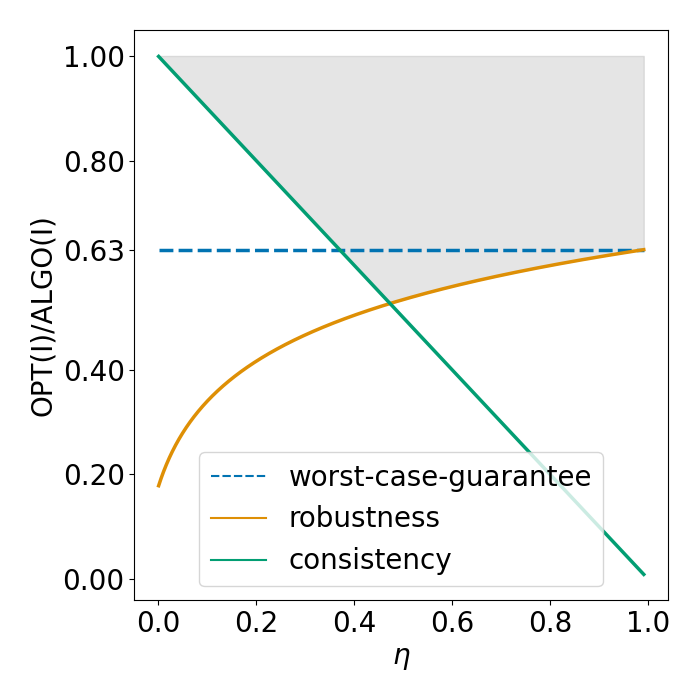
\includegraphics[width=0.4\textwidth]{../paper/Img/consistency_robustness.png}
	\end{center}
	\vspace{-1cm}
	\caption{Robustness-Consistency}
	\label{fig:robustness-consistency}
	\vspace{-0.2cm}
\end{wrapfigure}

\noindent In the figure, $\eta$ indicates the confidence in the predictions (or equivalently the error rate of predictions). The learning-augmented algorithm's performance bound is the maximum value of the green and orange curves (gray shaded area on the figure). We can observe that when $0.4 \leq \eta \leq 0.9$,
the algorithm's performance guarantee is worse than the classical worst-case guarantee (that can be achieved by simply ignoring all predictions).
Intuitively, in the case of neither very low nor very high confidence in the predictions, the algorithm has a hard time deciding if it should follow the predictions or the best-known standard algorithm in the worst-case paradigm.
It naturally raises the question whether we can achieve at least a constant factor of the worst-case guarantee (where the constant is as close to 1 as possible), while assuring a resilient output solution regardless of the predictions' quality.
Our algorithms with the new benchmark provides an answer to this question.


The paper of \cite{AnandGe22:Online-Algorithms} is the closest to ours, which also studies the design of algorithms with multiple experts.
They consider a \texttt{DYNAMIC} benchmark that is intuitively
the minimum cost solution that is supported by at least one expert solution at each time step. Formally:
\[\texttt{DYNAMIC} = \min_{\hat{\textbf{x}} \in \hat{X}} \sum_{i=1}^{n} c_i \hat{x}_i \textnormal{, where}\]
%
\[\hat{X} = \{\hat{\vect{x}} : \forall\ i \in [n],\ \forall\ t \in [T],\ \exists\ k \in [K]\ \textnormal{ such that } s_{i,k}^{t} \le \hat{x}_i \}\]
%
Our benchmark, \texttt{LIN-COMB}, is included in \texttt{DYNAMIC}, since every solution $x_{i}^{t}$ in \texttt{LIN-COMB} satisfies:
\[
	x_{i}^{t} \geq \sum_{k} s_{i,k}^{t}w_{k}^{t} \geq \min_{k} \{s_{i,k}^{t}\}
\]
therefore, for any $i$ and $t$, there exists $k$ such that $x_{i}^{t} \geq s_{i,k}^{t}$.
However, the inverse is not true: a solution $\hat{\vect{x}}^{t} \in \hat{X}$ in \texttt{DYNAMIC} is not necessarily
a linear combination of the experts' solutions.
The \texttt{DYNAMIC} benchmark in \cite{AnandGe22:Online-Algorithms} relied on the assumption that at every time step
the experts' solutions are tight. This assumption does not allow the representation of some realistic problems and it is impossible to maintain in online solutions (see Appendix~\ref{appix-tight-solutions}).
Further, \cite{AnandGe22:Online-Algorithms} claimed an $O(\ln(K))$-competitive algorithm in the \texttt{DYNAMIC} benchmark.
Unfortunately, their benchmark is too strong; we show an example in Appendix~\ref{sec:counter-example}
in which their algorithm's performance guarantee is unbounded in their \texttt{DYNAMIC}
benchmark. We believe that with a different benchmark their algorithm could be $O(\ln(K))$-competitive, however, we did not manage to prove this.


Integrating multiple predictions into online algorithms was a topic of other papers as well.
As an example, \cite{GollapudiPanigrahi19:skirental-multiple-predictions} studied the ski rental problem with multiple predictions.
The authors defined a consistency metric, which compares the performance of their algorithm to the optimal solution, given that at least one prediction (among the $k$ predictions) is optimal.
%By carefully integrating every prediction in their algorithm design, the authors managed to reduce the overall prediction error rate and obtain the best possible performance guarantee for their algorithm. During their analysis, they defined a consistency metric, which compares the performance of their algorithm to the optimal solution, given that at least one prediction (among the $k$ predictions) is correct.
\cite{AlmanzaChierichetti21:Online-Facility} also considered multiple predictions in the online facility location problem.
%The suggestions are treated as a family of sets and the authors use the union of these suggestions.
They compared the performance of their algorithm to the best possible solution obtained on the union of the suggestions. Recently, \cite{DinitzIm:Algorithms-with} studied the use of multiple predictors for several problems such as matching, load balancing, and non-clairvoyant scheduling. They provided algorithms competitive to the best predictor for such problems.
An important remark: all the above benchmarks are captured within \texttt{LIN-COMB}.

Furthermore, \cite{AntoniosEtAll23:mixing-predictions-metric-algorithms} proposed an algorithm with multiple experts for the metrical task system problem. Their benchmark allows switching from one expert to another at each time step, but it does not allow combinations of experts or any solution not suggested by one of the experts. In our \texttt{LIN-COMB} benchmark, the linear combinations that evolve over time could result in a solution that is not suggested by one of the experts and potentially, they can be much more efficient. In \cite{AntoniosEtAll23:mixing-predictions-metric-algorithms} there is a cost for state transitions, which is appropriate for their problems, but in many other problems, the smooth transition with additional costs from previous decisions to new ones is not allowed (past decisions are immutable). Therefore, the results of \cite{AntoniosEtAll23:mixing-predictions-metric-algorithms} are not applicable to our setting.

Combining online algorithms into a new algorithm to achieve better results than the individual input algorithms has been a long-standing online algorithm design question \cite{AzarBroder93:On-line-Choice,BlumBurch00:On-line-Learning}.
Its intrinsic difficulty is similar to the issue we mentioned earlier: when the performance of the given input algorithms (or heuristics) is unclear (especially in the online setting), it is challenging to create a combination that can surpass the performance of the included algorithms.
Following the current development of online algorithm design techniques with multiple predictions, this subject has been renewed with different machine learning approaches. Our paper contributes to this line of research.

\subsection{Paper overview}

In this paper we show two algorithms to solve online \emph{linear} and online \emph{convex} covering problems with multiple experts. While the convex setting includes the linear one, our proposed algorithm is simpler for the linear case. Therefore, \cref{sec:covering} details our first algorithm for the linear case, and afterwards, in \cref{sec:convex} we detail the extension to the convex case. \cref{sec:exp} shows empirical results, and we conclude in \cref{sec:conclusion}.
%!TEX root = ./main.tex

\section{The framework}		\label{sec:covering}

\subsection{Formulation}
We formulate the online covering problem that we described in the Preliminaries as a problem of finding the minimum cost solution among all the possible solutions. This formulation has an exponential number of variables and constraints; however, it allows us to transform the non-linear objective function into a linear one, which is crucial for our algorithm and proofs.

Let $S \subseteq \mathcal{E}$ be a \emph{solution} if $\one_{S}$ corresponds to a feasible solution. Let $x_{e}$ be a variable indicating whether resource $e$ is selected.
Let $z_{S}$ be an indicator variable for solution $S$. If $z_{S} = 1$, then every variable
$x_{e} = 1$ if $e \in S$, and $x_{e} = 0$ if $e \notin S$. Otherwise, $z_S = 0$. In other words, $z_{S} = 1$ if and only if $\one_{S}$ is the selected solution of the online covering problem. At each time step~$t$ during the execution, a new constraint is revealed. For every subset $A \subseteq \mathcal{E}$, we define the value $c^{t}(A) := \max\{0,\ 1 - \sum_{e \in A} a^{t}_{e}\}$, to be the amount we need until constraint satisfaction. Given this value, we normalize the constraint coefficients to be $a^{t}_{e}(A) := \min\{a_{e}^{t},\ c^{t}(A)\}$. Finally, we define $b^{t}_{e}(A) := a^{t}_{e}(A)\ /\ c^{t}(A)$ where $c^{t}(A) > 0$. The values $b^{t}_{e}(A)$ correspond to the coefficients in the knapsack inequality constraints \citep{CarrFleischer:2000}. The primal and dual programs are:

\vspace{-0.6cm}
\begin{minipage}[t]{0.45\textwidth}
	\begin{align*}
		\min  \sum_{S \subseteq \mathcal{E}} &f(\one_{S})\ z_{S} \\
		\sum_{e \notin A} b_{e}^{t}(A) \ x_{e} &\geq 1 & &  \forall t,\ \forall A \subseteq \mathcal{E} \\
		\sum_{S: e \in S} z_{S}  &= x_{e}	& & \forall e \\
		\sum_{S \subseteq \mathcal{E}} z_{S} &= 1 & & \\
		x_{e}, z_{S} &\in \{0,1\} & & \forall e,\ \forall S \subseteq \mathcal{E}\\
	\end{align*}
\end{minipage}
\quad
\begin{minipage}[t]{0.5\textwidth}
	\begin{align*}
		\max \sum_{t, A} \alpha^{t}_{A} &+ \gamma \\
		\sum_{t} \sum_{A: e \notin A} b_{e}^{t}(A) \ \alpha_{A}^{t} &\leq \beta_{e}  & &  \forall e \\
		\gamma + \sum_{e \in S} \beta_{e} &\leq f(\one_{S})  & & \forall S \subseteq \mathcal{E}\\
		\alpha^{t}_{A} &\geq 0 & & \forall t,\ \forall A \subseteq \mathcal{E}\\
		\beta_e &\geq 0 & & \forall e\\
		\gamma &\geq 0 & &
	\end{align*}
\end{minipage}
\vspace{-0.6cm}

In the primal program, the first constraints are knapsack-constraints \citep{CarrFleischer:2000} of the given polytope, and they are equivalent to $\sum_{e \notin A} a_{e}^{t}(A) \ x_{e} \geq c^{t}(A)$. It is sufficient to satisfy constraints where $c^{t}(A) > 0$. The second primal constrain ensures that if a resource $e$ is chosen, the selected solution must contain $e$.
The third constraint guarantees that \emph{one} solution is selected.

\subsection{Algorithm}
In our proposed algorithm, $\vect{x} \in [0, 1]^{|\mathcal{E}|}$ corresponds to the current solution of the algorithm. During the execution, we rely on the objective function's multilinear extension $F$, parametrized by $\lambda$ and $\mu$. We assume, that $F(\vect{x})$ is $(\lambda, C \mu)$-locally-smooth, where $C$ is a constant that arises from the algorithm's analysis (see Lemma~\ref{lem:prim-dual-feasible}). Algorithm~\ref{algo:covering} follows the scheme of \cite{Thang20:Online-Primal-Dual}, which uses both the primal and dual variables to solve the problem.

We have two notions of time in our algorithm. First, at each discrete time step $t$, a new primal constraint arrives. Second, we have a continuous time $\tau$ throughout the execution. The solution of the algorithm increases gradually with time $\tau$.  To simplify the notations, when the context only uses the current time of the execution, $\vect{x}$ refers to $\vect{x}(\tau)$, the current solution at time $\tau$.

\begin{algorithm}[!ht]
	\begin{algorithmic}[1]
	\STATE Initially, set $A^* \gets \emptyset$ \ \ \texttt{(where $A^*$ is the solution set and $\forall e \in A^* : x_{e} = 1$)}
	\STATE All primal and dual variables are initially set to 0
	\STATE During every step, for each feasible solution $S$, $z_{S} = \prod_{e \in S} x_{e} \prod_{e \notin S} (1 - x_{e})$ is maintained.
	\STATE Let $\tau$ be the continuous timer during the execution of the algorithm.
	\FOR{each time $t$, for the new primal constraint $\sum_{e} a_{e}^{t} x_{e} \geq 1$
	and dual variable $\alpha^{t}_{A^*}$}
		\WHILE[\texttt{Increase primal, dual variables}]{$\sum_{e \notin A^{*}} b^{t}_{e}(A^{*})\ x_{e} < 1$}
			\STATE Increase $\tau$ with a rate of $1$.
			\STATE Increase $\alpha^{t}_{A^{*}}$ at rate $1\ /\ (\lambda \ \ln(1+2d^{2}/\eta))$
			%(Note that $c_{k,A^{*}} > 0$ by the condition of the while loop.)
			\label{algo-covering:alpha}
			\FOR{$e \notin A^{*}$ such that $b^{t}_{e}(A^{*}) > 0$}
				\STATE \textbf{if} $\beta_{e} <  \frac{1}{\lambda} \nabla_{e} F(\vect{x})$ \textbf{then}
				$\beta_{e} \gets \frac{1}{\lambda} \nabla_{e} F(\vect{x})$
				\label{algo-covering:beta}
				\STATE Increase $x_{e}$ at a rate according to the following
				\begin{align*}
					\frac{\partial x_{e}}{\partial \tau}	\gets
					\frac{b^{t}_{e}(A^{*}) \ x_{e}}{\lambda \beta_{e}} + \frac{\eta}{\lambda \beta_{e} d}
					+ \frac{(1 - \eta) \cdot \one_{\{pred(x_{e}) = 1\}}}{\nabla_{e} F(\vect{x}) \cdot |\{e': pred(x_{e'}) = 1,\ b^{t}_{e'}(A^{*}) > 0\}| }
				\end{align*}
				\label{algo-covering:x}
			\ENDFOR
			\STATE \textbf{if} $x_{e} = 1$ \textbf{then} $A^{*} \gets A^{*} \cup \{e\}$
			\FOR[\texttt{Decrease dual variables}]{$e : e \notin A^*$} \label{algo-decrease}
				\WHILE{
					$\sum_{t'=1}^{t} \sum_{A: e \notin A} b^{t'}_{e}(A) \ \alpha^{t'}_{A} > \beta_{e}$}
						\FOR{$(t_{e}^{*}, A) \textnormal{ such that } b^{t_{e}^{*}}_{e}(A) =  \max \{b^{t'}_{e}(A)\ |\ \forall A: e \notin A \textnormal{ and }\forall t' \leq t \textnormal{ s.t. } \alpha^{t'}_{A} > 0\}$} \label{algo-covering:bmax}
							\STATE Decrease $\alpha^{t_{e}^{*}}_{A}$ continuously with a rate of
							$\frac{b^{t}_{e}(A^{*})}{b^{t_{e}^{*}}_{e}(A)} \cdot\frac{1}{\lambda \cdot \ln(1+2d^{2}/\eta)}$
							\label{algo-covering:decrease}
					\ENDFOR
				\ENDWHILE
			\ENDFOR
		\ENDWHILE
	\ENDFOR
	\end{algorithmic}
	\caption{Online Algorithm for Non-Linear Covering Problems.}
	\label{algo:covering}
\end{algorithm}

When a new primal constraint arrives, the current dual variable $\alpha^{t}_{A^*}$ increases at a constant rate (line \ref{algo-covering:alpha}), while the $\beta_e$ variables are updated according to the partial derivative of the mulitlinear extension (line \ref{algo-covering:beta}). We note a subtle point here: if $\beta_e < \frac{1}{\lambda} \nabla_{e} F(\vect{x})$ then we set
$\beta_e = \frac{1}{\lambda} \nabla_{e} F(\vect{x})$, but if $\beta_e > \frac{1}{\lambda} \nabla_{e} F(\vect{x})$ then we do not change the value of $\beta_e$. This update preserves the following invariants during the execution of the algorithm: $\beta_{e} \geq \frac{1}{\lambda} \nabla_{e} F(\vect{x})$ and $\beta_{e}$ is non-decreasing. (Remark: if $\nabla_{e} F(\vect{x})$ is monotone on every coordinate $e$, then it is sufficient to always set $\beta_{e} \gets \frac{1}{\lambda} \nabla_{e} F(\vect{x})$.)

The update on line \ref{algo-covering:x} is inspired by the multiplicative weight update method (where the increasing rate of $x_{e}$
is inversely proportional to $\beta_{e}$) and the updating approach of \cite{BamasMaggiori20:The-Primal-Dual-method}. The oracle's prediction skews the weights to assign more value to the predicted coordinates $x$.
Starting from line \ref{algo-decrease}, the algorithm decreases some of the dual variables using a similar idea as in
\cite{AzarBuchbinder16:Online-Algorithms}. This decrease is necessary to maintain the feasibility of the dual solution.

\subsection{Primal and dual variables}
Let $\vect{x}(\tau)$ be the algorithm's primal solution at time $\tau$. The dual variables $\alpha^{t}_{A}$ and $\beta_{e}$ are assigned during the execution, but not $\gamma$. To make the dual solution feasible, we set $\gamma = -\frac{\mu}{4\lambda \cdot \ln(1+2d^{2}/\eta)} F(\vect{x}(\tau))$ (see Lemma~\ref{lem:prim-dual-feasible}). Each $\beta_{e} = \frac{1}{\lambda} \nabla_{e} F(\vect{x}(\tau'))$, for some primal solution $\vect{x}(\tau')$, where $\tau' \le \tau$. Moreover, $\vect{x}(\tau) \geq \bigvee_{\tau' \le \tau} \vect{x}(\tau')$ (each coordinate $x_{e}(\tau) = \max_{\tau' \le \tau}\{x_{e}(\tau')\}$), since the $x_e$-variables are non-decreasing. Consequently, each $\beta_{e} \geq \frac{1}{\lambda} \nabla_{e} F(\vect{x}(\tau))$. Using these properties, Lemma~\ref{lem:bound-x} gives a lower bound on $\vect{x}(\tau)$. We highlight that the proof if this lemma does \emph{not} require the gradient of $F$ to be monotone.
(With this assumption, the algorithm can set $\beta_{e} = \frac{1}{\lambda} \nabla_{e} F(\vect{x}(\tau))$ at each step $\tau$ of the execution.)

\setcounter{theorem}{0}
\begin{restatable}{lemma}{BoundX}
\label{lem:bound-x}
Let $e$ be an arbitrary resource.
At any moment $\tau$ during the execution of the algorithm,
when $t$ constraints have already been released, it always holds that
$$
x_{e}	\geq  \frac{\eta}{b^{t_{e}^{*}}_{e}(A) \ d}
		\left[ \exp\biggl( \frac{\ln(1+2d^{2}/\eta)}{\beta_{e}}
				\cdot \sum_{A: e \notin A} \sum_{t' \le t} b^{t'}_{e}(A) \cdot \alpha^{t'}_{A} \biggr) - 1 \right]
$$
where $b^{t_{e}^{*}}_{e}(A)$ is defined in the algorithm on line~\ref{algo-covering:bmax}.
\end{restatable}
\begin{proof}
	The proof is available in \cref{apix:lemma-proof}.
\end{proof}
%
\begin{lemma} \label{lem:prim-dual-feasible}
The primal and dual variables are feasible.
\end{lemma}
%
\begin{proof}

\textbf{Primal feasibility.}
While a primal covering constraint is unsatisfied, the $x_e$-variables are increasing. At the end of the first iteration, the first primal covering constraint is satisfied. Afterwards, the new constraints are
also satisfied, since the algorithms maintains $z_{S} = \prod_{e \in S} x_{e} \prod_{e \notin S} (1 - x_{e})$.
If we choose an element $e$ with probability $x_{e}$, then $z_{S}$ is the probability
that the set of selected items is $S$. Therefore, the total probability $\sum_{S} z_{S} = 1$. By a similar argument, we get the following:
\[
	\sum_{S: e \in S} z_{S} = x_{e} \sum_{S' \subseteq E \setminus \{e\}} \prod_{e' \in S'} x_{e'} \prod_{e' \notin S'} (1 - x_{e'}) = x_{e}
\]
since
\[
	\sum_{S' \subseteq E \setminus \{e\}} \prod_{e' \in S'} x_{e'} \prod_{e' \notin S'} (1 - x_{e'}) = 1
\].

\textbf{Dual feasibility.} Let us now prove that the first dual constraint is always satisfied during the execution. The algorithm maintains $\sum_{t' \le t} \sum_{A: e \notin A} b^{t'}_{e}(A)\ \alpha^{t'}_{A} \leq \beta_{e}$. % (strict inequality happens only if $x_{e} = 1$).
Whenever this inequality is violated, the algorithm decreases (see line \ref{algo-covering:decrease}) some of the $\alpha$-variables in a way that the increasing rate of $\sum_{t' \le t} \sum_{A: e \notin A} b^{t'}_{e}(A)\ \alpha^{t'}_{A}$ is at most 0. By the $\beta$-variables' definition, the first dual constraint holds.

Let us consider the second dual constraint. Let $\vect{x}(\tau)$ be the final solution of the algorithm. For each fixed resource $e$, the value $\beta_{e} = \frac{1}{\lambda} \nabla_{e} F(\vect{x}(\tau_e))$ for some previous solution $\vect{x}(\tau_e)$ where $\tau_e \le \tau$ and where $x_{e}(\tau_e) \leq x_{e}(\tau)$ for all $e$.
Let $\vect{y} := \bigvee_{\tau' \le \tau} \vect{x}(\tau') \leq \vect{x}(\tau)$, so for each coordinate $e$ of $\vect{y}$, we have $y_{e} = \max_{\tau' \le \tau}\{x_{e}(\tau')\}$.
By definition of the dual variables, the second dual constraint (after rearranging the terms) reads
\begin{align*}
	\frac{1}{\lambda} \sum_{e \in S} \nabla_{e} F(\vect{x}(\tau_e)) \leq F(\one_{S}) + \frac{\mu}{4\lambda \cdot \ln(1+2d^{2}/\eta)} F(\vect{x}(\tau)) \quad \quad \forall\ S \subseteq \mathcal{E}
\end{align*}
since we set $\gamma = -\frac{\mu}{4\lambda \cdot \ln(1+2d^{2}/\eta)} F(\vect{x}(\tau))$, and $\vect{x}(\tau_e)$ corresponds to the solution during the execution where $\beta_e$ was set to $\frac{1}{\lambda} \nabla_{e} F(\vect{x}(\tau_e))$.
Since $F$ is monotone, $F(\vect{x}(\tau)) \geq F(\vect{y})$. To prove that the above inequality holds, it is sufficient to show that
\begin{align*}
	\frac{1}{\lambda} \sum_{e \in S} \nabla_{e} F(\vect{x}(\tau_e)) \leq F(\one_{S}) + \frac{\mu}{4\lambda \cdot \ln(1+2d^{2}/\eta)} F(\vect{y})
\end{align*}
which means that $F$ needs to be  $\bigl(\lambda, \frac{\mu}{4\ln(1+2d^{2}/\eta)}\bigr)$-locally-smooth. Our initial assumption was that $F$ is $(\lambda, C \mu)$-locally-smooth. By setting $C := \frac{1}{4\ln(1+2d^{2}/\eta)}$, the lemma holds.
\end{proof}

\setcounter{theorem}{0}
\begin{theorem} \label{thm:covering-formal}
	Let $F$ be the multilinear extension of the online non-linear covering problem's objective function $f$ and
	$d$ be the maximal row sparsity of the constraint matrix (formally $d = \max_{t \le T} |\{a^{t}_{e}: a^{t}_{e} > 0\}|$).
	Assuming that $F$ is $\bigl(\lambda, \frac{\mu}{\ln(1+2d^{2}/\eta)}\bigr)$-locally-smooth
	for some parameters ($\lambda > 0$, $\mu < 1$ and $0 < \eta \leq 1$), there exists an $O\bigl( \frac{1}{1 - \eta} \bigr)$-consistent and $O\bigl( \frac{\lambda}{1 - \mu}  \cdot \ln \frac{d}{\eta} \bigr)$-robust algorithm for any $\eta \in (0,1]$ which produces a fractional solution for the given problem.
\end{theorem}
\begin{proof}

\textbf{Robustness.}
By bounding the increases of the primal and dual objective values at any time $\tau$ during the execution of
Algorithm~\ref{algo:covering}, we can determine the robustness. Upon the release of the $t^{\text{th}}$ constraint,
let $A^{*}$ be the current solution with the chosen set of resources $e$ such that $x_{e} = 1$.

\noindent The derivative of the primal objective function with respect to $\tau$ is:
%
\begin{align}	\label{eq:covering-primal}
\sum_{e \in \mathcal{E}} & \nabla_{e} F(\vect{x}) \cdot \frac{\partial x_{e}}{ \partial \tau} \notag \\
&= \sum_{e\ :\ b^{t}_{e}(A^{*})\ >\ 0} \nabla_{e} F(\vect{x})
	\ \left( \frac{b^{t}_{e}(A^{*}) \ x_{e}}{\lambda\ \beta_{e}} + \frac{\eta}{\lambda\ \beta_{e}\ d}
		 + \frac{(1 - \eta) \ \one_{\{pred(x_{e})\ =\ 1\}}}{\nabla_{e} F(\vect{x}) \cdot |\{e': pred(x_{e'})\ =\ 1,\ b^{t}_{e'}(A^{*}) > 0\}| }
 \right)	\notag \\
%
&\leq  \sum_{e\ :\ b^{t}_{e}(A^{*})\ >\ 0} \biggl( b^{t}_{e}(A^{*}) \ x_{e} + \frac{\eta}{d} \biggr)
	+ \sum_{e\ :\ pred(x_e)\ =\ 1 \atop b^{t}_{e}(A^{*})\ >\ 0} \frac{(1 - \eta)}{ |\{e': pred(x_{e'}) = 1,\ b^{t}_{e'}(A^{*}) > 0\}|  } \notag \\
& \leq 2
\end{align}
The first inequality follows $\nabla_{e} F(\vect{x}) \leq \lambda \  \beta_{e}$. The second inequality is
due to the definition of $d$ and  the fact that
$\sum_{e \notin A^{*}} b^{t}_{e}(A^{*}) \ x_{e} \leq 1$ always holds during the algorithm. (The number of $b^{t}_{e}(A^{*})$ values which are strictly greater than 0, is at most $d$.)

At any time $\tau$, let $U(\tau)$ be the set of resources $e$ such that
$\sum_{t' \le t} \sum_{A: e \notin A} b^{t'}_{e}(A)\ \alpha^{t'}_{A} = \beta_{e}$ and $b^{t}_{e}(A^*) > 0$.
Note that $|U(\tau)| \leq d$ by definition of $d$.
As long as $\sum_{e \notin A^{*}} b^{t}_{e}(A^*)\ x_{e}  < 1$,
using Lemma~\ref{lem:bound-x} we get that for every $e \in U(\tau)$,
%
\begin{align*}
\frac{1}{b^{t}_{e}(A^*)} > x_{e} \geq \frac{\eta}{b^{t_{e}^{*}}_{e}(A) \ d}
				\left[ \exp\biggl(\ln(1+2d^{2}/\eta) \biggr) - 1 \right]
				= \frac{2 d}{b^{t_{e}^{*}}_{e}(A)}
\end{align*}
where $b^{t_{e}^{*}}_{e}(A)$ is defined in the algorithm on line~\ref{algo-covering:bmax}.
Therefore, $\frac{b^{t}_{e}(A^{*})}{b^{t_{e}^{*}}_{e}(A)} \leq \frac{1}{2d}$. Following the definition of $U(\tau)$, we can bound the increase of the dual at time $\tau$.

\noindent The derivative of the dual with respect to $t$ is:
\begin{align*}
\frac{\partial D}{\partial \tau}
&=  \sum_{t' \le t} \sum_{A : e \notin A} \frac{\partial \alpha^{t'}_{A}}{\partial \tau} + \frac{\partial \gamma}{\partial \tau}
= \sum_{t' \le t} c^{t'}(A^{*}) \cdot \frac{\partial \alpha^{t'}_{A^{*}}}{\partial \tau} + \frac{\partial \gamma}{\partial \tau} \\
&= \frac{1}{\lambda \cdot \ln(1 + 2d^{2}/\eta)} \cdot \biggl(1 - \sum_{e \in U(\tau)} \frac{b^{t}_{e}(A^{*})}{b^{t_{e}^{*}}_{e}(A)} \biggr)
	- \frac{\mu}{4\lambda \cdot \ln(1 + 2d^{2}/\eta)} \cdot \sum_{e} \nabla_{e} F(\vect{x}) \frac{\partial x_{e}}{\partial \tau} \\
%
&\geq \frac{1}{\lambda \cdot \ln(1 + 2d^{2}/\eta)} \biggl(1 - \sum_{e \in U(\tau)} \frac{1}{2d} \biggr)
	- \frac{\mu}{2 \lambda \cdot \ln(1 + 2d^{2}/\eta)} \\
%
&\geq \frac{1 - \mu}{2 \lambda \cdot \ln(1 + 2d^{2}/\eta)}.
\end{align*}
The third equality holds since $\alpha^{t}_{A^{*}}$ is increased and other $\alpha$-variables in
$U(\tau)$ are decreased. The first inequality uses the fact that $\frac{b^{t}_{e}(A^{*})}{b^{t_{e}^{*}}_{e}(A)} \leq \frac{1}{2d}$
and Inequality~(\ref{eq:covering-primal}).
The last inequality holds since $|U(\tau)| \leq d$.
Hence, the robustness is at least $\frac{4 \lambda}{1 - \mu} \cdot \ln(1 + 2d^{2}/\eta)$.

\textbf{Consistency.} We establish consistency with a similar argument as \cite{BamasMaggiori20:The-Primal-Dual-method}.
Considering an arbitrary moment $\tau$ during the algorithm's execution, let $S_{1} = S_{1}(\tau)$ be the set of resources selected by the prediction. Formally, $\forall\ e \in S_{1} : pred(x_{e}) = 1$ up to time $\tau$. Let $S_{2} = S_{2}(\tau)$ contain the remaining resources.
The primal objective increase due to $S_{1}$ and $S_{2}$:

\begin{align*}
\sum_{e \in S_{1}} \nabla_{e} F(\vect{x})\ \frac{\partial x_{e}}{ \partial \tau}
&= \sum_{e \in S_{1}} \nabla_{e} F(\vect{x})
	\ \left( \frac{b^{t}_{e}(A^{*}) \ x_{e}}{\lambda\ \beta_{e}} + \frac{\eta}{\lambda\ \beta_{e}\ d}
		 + \frac{(1 - \eta)}{\nabla_{e} F(\vect{x}) \cdot |\{e': pred(x_{e'}) = 1\}| }
 \right)\\
 &\geq 1 - \eta \\
 %
 \sum_{e \in S_{2}} \nabla_{e} F(\vect{x})\ \frac{\partial x_{e}}{ \partial \tau}
&= \sum_{e \in S_{2}} \nabla_{e} F(\vect{x})
	\ \left( \frac{b^{t}_{e}(A^{*}) \ x_{e}}{\lambda\ \beta_{e}} + \frac{\eta}{\lambda\ \beta_{e}\ d} \right)
\leq 1 + \eta
\end{align*}
Therefore, the primal objective increase is at most $\bigl(1 +  \frac{1 + \eta}{1 - \eta} \bigr)$ time the increase restricted to
the set~$S_{1}$. Moreover, the algorithm's primal objective value restricted to $S_{1}$ is smaller than
the prediction's, since $\forall e \in S_{1} : x_{e} \leq 1 = pred(x_{e}$).
We can deduce that the algorithm is $O\bigl( \frac{1}{1 - \eta} \bigr)$-consistent with the prediction.
\end{proof}

%!TEX root = ./main.tex

\section{Applications}	\label{sec:app}
\setcounter{theorem}{5}

%%!TEX root = ./main.tex

\subsection{Norm minimization} \label{appix-norm}

In this section, we consider the $\ell_{k}$-norm function as the objective, i.e.,  $f(\vect{x}) = \|C \vect{x}\|_{k}$ where $C \in \mathbb{R}^{m \times n}$ is a matrix. 
Specifically, the corresponding optimization problem is: $\min \|C \vect{x}\|_{k}$ subject to $B \vect{x} \geq 0$. 

To apply our framework, we first determine the smoothness parameters of $\|C \vect{x}\|_{k}$.

\begin{lemma} \label{lem-makespan}
For $C \in \mathbb{R}^{m \times n}$, function $f(\vect{x}) := \|C \vect{x}\|_{k}$ is $(k,0)$-locally-smooth.
\end{lemma}
%
\begin{proof}
We prove that, for every subset $S \subseteq \{1, \ldots, n\}$ and for every $\vect{x} \in [0,1]^{n}$, it holds that
%
\begin{align}	\label{ineq:lp-smooth}
\sum_{e \in S} \nabla_{e} f(\vect{x}) \leq  k \cdot \|C \vect{x}\|_{k} 
\end{align}


We have
%
\begin{align*}
\frac{\partial f(x)}{\partial x_{e}}
= k \cdot \sum_{i = 1}^{m} \frac{c_{i,e} \cdot \bigl( \sum_{e' = 1}^{n} c_{i,e'} x_{i,e'} \bigr)^{k-1} }{ \left[ \sum_{i' = 1}^{m} 
		\bigl( \sum_{e'= 1}^{n} c_{i',e'} x_{i',e'} \bigr)^{k} \right]^{(k-1)/k}}
\end{align*}
Hence,
\begin{align*}
\sum_{e \in S} \frac{\partial f(x)}{\partial x_{e}}
= k \cdot \frac{ \sum_{e \in S} \sum_{i = 1}^{m} c_{i,e} \cdot \bigl( \sum_{e' = 1}^{n} c_{i,e'} x_{i,e'} \bigr)^{k-1} }{ \left[ \sum_{i' = 1}^{m} \bigl( \sum_{e'= 1}^{n} c_{i',e'} x_{i',e'} \bigr)^{k} \right]^{(k-1)/k}}
\end{align*}

Inequality (\ref{ineq:lp-smooth}) is equivalent to
\begin{align*}
\frac{ \sum_{e \in S} \sum_{i = 1}^{m} c_{i,e} \cdot \bigl( \sum_{e' = 1}^{n} c_{i,e'} x_{i,e'} \bigr)^{k-1} }{ \left[ \sum_{i' = 1}^{m} \bigl( \sum_{e'= 1}^{n} c_{i',e'} x_{i',e'} \bigr)^{k} \right]^{(k-1)/k}}
	\leq   \biggl \| \biggl( \sum_{e: e \in S} c_{1,e},\ \ldots\ , \sum_{e: e \in S} c_{m,e}  \biggr) \biggr \|_{k}
\end{align*}
%
By multiplying both sides with the denominator of the left-hand side, it is equivalent to:
%
\begin{align*}
\sum_{e \in S} \sum_{i = 1}^{m} c_{i,e} \cdot \bigl( \sum_{e' = 1}^{n} c_{i,e'} x_{i,e'} \bigr)^{k-1}  
&\leq
        \left ( \sum_{i'=1}^{m} \biggl [ \biggl( \sum_{e'= 1}^{n} c_{i',e'} x_{i',e'} \biggr)^{k-1} \biggr ]^{k/(k-1)} \right )^{(k-1)/k} \\
        			& \qquad \cdot \biggl \| \biggl( \sum_{e: e \in S} c_{1,e}, \ \ldots\ , \sum_{e: e \in S} c_{m,e}  \biggr) \biggr \|_{p} \\
    %
%& \Updownarrow \\
    %
 \Leftrightarrow \quad  \sum_{i=1}^{m} \biggl( \sum_{e: e \in S} c_{i,e} \biggr) \cdot \biggl( \sum_{e'=1}^{n} c_{i,e'} x_{i,e'} \biggr)^{k-1} 
 &\leq
        \left \| \left( \biggl( \sum_{e'=1}^{n} c_{1,e'} x_{1,e'} \biggr)^{k-1}, \ldots, \biggl( \sum_{e'=1}^{n} c_{m,e'} x_{m,e'} \biggr)^{k-1} \right)   \right \|_{\frac{k}{k-1}} \\
        		& \qquad \cdot \biggl \| \left( \biggl(\sum_{e: e \in S} c_{1,e} \biggr) ,.., \biggl( \sum_{e: e \in S} c_{m,e}\biggr)  \right) \biggr \|_{k}
\end{align*}
The above inequality holds by H\"older inequality ($\| a \cdot b\|_{1} \leq \| a \|_{p} \cdot \| b \|_{q}$ where $1/p + 1/q = 1$).
Therefore, the lemma holds.
\end{proof}

The following theorem follows immediately from our framework.

\begin{proposition}	\label{prop:norm}
Algorithm~\ref{algo:covering} gives a
$O(\frac{1}{1 - \eta})$-consistent and $O\bigl( k \cdot \log (d/\eta)\bigr)$-robust fractional solution
for the problem of minimizing $\|C \vect{x}\|_{k}$ under covering constraints.
\end{proposition}

This result implies that in the classic online setting (without predictions, i.e., $\eta = 1$), Algorithm~\ref{algo:covering} 
achieves the asymptotically \emph{optimal} competitive ratio of  $O\bigl( k \cdot \log (d)\bigr)$ 
for the problem of minimizing $\|C \vect{x}\|_{k}$ under covering constraints (due to the lower bound 
of $\Omega\bigl( k \cdot \log (d)\bigr)$ in \cite{AzarCohen14:Online-Covering}).

\subsection{Online mixed packing and covering constraints.}
In this section, we consider the online mixed packing and covering problem (OMPC) studied in \cite{AzarBhaskar13:Online-mixed}. 
Given a set of packing constraints $C \vect{x} \leq \vect{1}$ (where $C \in \mathbb{R}^{m \times n}$), 
and a set of covering constraints $B \vect{x} \geq \vect{1}$, with positive coefficients, 
such that the packing constraints are known in advance, and the covering constraints arrive one at a time. 
The goal is that after the arrival of each
covering constraint, increase $\vect{x} \geq \vect{0}$ so that the new covering constraint is satisfied and the factor $\xi$
by which $C \vect{x} \leq \xi \cdot \vect{1}$ is as small as possible.

This problem can formalized as: $\min \| C \vect{x}\|_{\infty}$ subject to online constraints $B \vect{x} \geq \vect{1}$. 
As $\ell_{\log m}$-norm is a constant approximation for $\ell_{\infty}$-norm, one can replace the objective as $\min \| C \vect{x}\|_{\log m}$. 
As a corollary of Proposition~\ref{prop:norm}, we get a fractional solution that is 
$O(\frac{1}{1 - \eta})$-consistent and $O\bigl( \log k \cdot \log (d/\eta)\bigr)$-robust for OMPC. 
Moreover, in the claissic online setting, the algorithm is $O\bigl( \log m \cdot \log d \bigr)$-competitive, i.e, \emph{optimal} up to a constant factor 
by a lower bound of $O\bigl( \log m \cdot \log d \bigr)$ in \cite{AzarBhaskar13:Online-mixed}.


\subsection{Norm minimization} 	\label{appix-norm}

As a first application, we consider problems where the objective function is the $\ell_{k}$-norm. Formally,  $f(\vect{x}) = \|C \vect{x}\|_{k}$, where $C \in \mathbb{R}_{+}^{m \times n}$ is a matrix with non-negative coefficients. The corresponding optimization problem is: $\min \|C \vect{x}\|_{k}$ subject to $B \vect{x} \geq 0$. To apply our framework, we first determine the $(\lambda, \mu)$-local-smoothness parameters of $\|C \vect{x}\|_{k}$.

\begin{lemma} \label{lem-makespan}
For $C \in \mathbb{R}^{m \times n}$, function $f(\vect{x}) := \|C \vect{x}\|_{k}$ is $(k,0)$-locally-smooth.
\end{lemma}
%
\begin{proof}
To prove the lemma, we show that for every subset $S \subseteq \{1, \ldots, n\}$ and for every $\vect{x} \in [0,1]^{n}$, the following holds.
%
\begin{align}	\label{ineq:lp-smooth}
\sum_{e \in S} \nabla_{e} f(\vect{x}) \leq  k \cdot \|C \cdot \one_{S}\|_{k}
\end{align}
%
The partial derivative is
%
\begin{align*}
\frac{\partial f(\vect{x})}{\partial x_{e}}
= k \cdot \sum_{i = 1}^{m} \frac{c_{i,e} \cdot \bigl( \sum_{e' = 1}^{n} c_{i,e'} x_{i,e'} \bigr)^{k-1} }{ \left[ \sum_{i' = 1}^{m}
		\bigl( \sum_{e'= 1}^{n} c_{i',e'} x_{i',e'} \bigr)^{k} \right]^{(k-1)/k}},
\end{align*}
so when we sum over $S$, we get
\begin{align*}
\sum_{e \in S} \frac{\partial f(\vect{x})}{\partial x_{e}}
= k \cdot \frac{ \sum_{e \in S} \sum_{i = 1}^{m} c_{i,e} \cdot \bigl( \sum_{e' = 1}^{n} c_{i,e'} x_{i,e'} \bigr)^{k-1} }{ \left[ \sum_{i' = 1}^{m} \bigl( \sum_{e'= 1}^{n} c_{i',e'} x_{i',e'} \bigr)^{k} \right]^{(k-1)/k}}.
\end{align*}
%
Therefore, inequality (\ref{ineq:lp-smooth}) is equivalent to
\begin{align*}
\frac{ \sum_{e \in S} \sum_{i = 1}^{m} c_{i,e} \cdot \bigl( \sum_{e' = 1}^{n} c_{i,e'} x_{i,e'} \bigr)^{k-1} }{ \left[ \sum_{i' = 1}^{m} \bigl( \sum_{e'= 1}^{n} c_{i',e'} x_{i',e'} \bigr)^{k} \right]^{(k-1)/k}}
	\leq   \biggl \| \biggl( \sum_{e: e \in S} c_{1,e}, \ldots , \sum_{e: e \in S} c_{m,e}  \biggr) \biggr \|_{k}.
\end{align*}
%
By multiplying both sides with the denominator of the left-hand side, we get
%
\begin{align*}
    \sum_{e \in S} \sum_{i = 1}^{m} c_{i,e} \cdot & \left( \sum_{e' = 1}^{n} c_{i,e'} x_{i,e'} \right)^{k-1} \leq \\
    & \left[ \sum_{i'=1}^{m} \biggl( \biggl( \sum_{e'= 1}^{n} c_{i',e'} x_{i',e'} \biggr)^{k-1} \biggr)^{k/(k-1)} \right]^{(k-1)/k}
    	\cdot \biggl \| \biggl( \sum_{e: e \in S} c_{1,e}, \ldots , \sum_{e: e \in S} c_{m,e}  \biggr) \biggr \|_{k}
\end{align*}
which is equivalent to
\begin{align*}
    \sum_{i=1}^{m} & \biggl( \sum_{e: e \in S} c_{i,e} \biggr) \cdot \biggl( \sum_{e'=1}^{n} c_{i,e'} x_{i,e'} \biggr)^{k-1} \leq \\
    & \left \| \left( \biggl( \sum_{e'=1}^{n} c_{1,e'} x_{1,e'} \biggr)^{k-1}, \ldots, \biggl( \sum_{e'=1}^{n} c_{m,e'} x_{m,e'} \biggr)^{k-1} \right) \right \|_{\frac{k}{k-1}}
    		\cdot \biggl \| \biggl( \sum_{e: e \in S} c_{1,e}, \ldots , \sum_{e: e \in S} c_{m,e}  \biggr) \biggr \|_{k}
\end{align*}
The last inequality above is true by the H\"older inequality ($\| a \cdot b\|_{1} \leq \| a \|_{p} \cdot \| b \|_{q}$ where $1/p + 1/q = 1$), so the lemma holds.
\end{proof}

\begin{proposition}	\label{prop:norm}
Algorithm~\ref{algo:covering} gives an
$O(\frac{1}{1 - \eta})$-consistent and $O\bigl( k \cdot \log (d/\eta)\bigr)$-robust fractional solution
for the problem of minimizing $\|C \vect{x}\|_{k}$ under covering constraints.
\end{proposition}

\cref{prop:norm} follows immediately from our framework.
This result implies that in the standard online setting (which does not have predictions, so $\eta = 1$), Algorithm~\ref{algo:covering}
achieves the asymptotically \emph{optimal} competitive ratio of  $O\bigl( k \cdot \log (d)\bigr)$
for the problem of minimizing $\|C \vect{x}\|_{k}$ under covering constraints. (See the lower bound
of $\Omega\bigl( k \cdot \log (d)\bigr)$ in \cite{AzarCohen14:Online-Covering}.)

%%%%%%%%%%%%%%%%%%%%%%%%

\subsection{Online mixed packing and covering}	\label{appix-mixed}
In an online mixed packing and covering problem (studied in \cite{AzarBhaskar13:Online-mixed}),
we are given a set of packing constraints $C \vect{x} \leq \one$ (where $C \in \mathbb{R}^{m \times n}$),
and a set of covering constraints $B \vect{x} \geq \one$. The coefficients of all the constraints are positive,
and the packing constraints are known in advance, but the covering constraints arrive one at a time.
The goal is to increase $\vect{x} \geq \mathbb{0}$ after the arrival of each covering constraint
such that the new constraint is satisfied and the factor~$\xi$ by which $C \vect{x} \leq \xi \cdot \one$ is as small as possible. In other words, we want to satisfy the covering constraints that arrive online with the smallest possible packing constraint violation.

This problem can be formalized as: $\min \| C \vect{x}\|_{\infty}$ subject to online constraints $B \vect{x} \geq \one$.
As the $\ell_{\log m}$-norm is a constant approximation for the $\ell_{\infty}$-norm, we can replace the objective with $\min \| C \vect{x}\|_{\log m}$.
As a corollary of Proposition~\ref{prop:norm}, we get a fractional solution that is
$O(\frac{1}{1 - \eta})$-consistent and $O\bigl( \log k \cdot \log (d/\eta)\bigr)$-robust.
Moreover, in the standard online setting, our algorithm is $O\bigl( \log m \cdot \log d \bigr)$-competitive. This is \emph{optimal} up to a constant factor
due to the lower bound of $O\bigl( \log m \cdot \log d \bigr)$ in \cite{AzarBhaskar13:Online-mixed}.



%\subsection{Load Balancing}
%
%Load balancing is a classic problem in discrete optimization with wide-ranging applications (for example, resource management in data centres).
%This problem revolves around assigning jobs that arrive online to $m$ available unrelated machines while minimizing their maximum load.
%Each arriving job $j$ reveals its machine dependent execution time $p_{ij}$ where $i \in \{1, m\}$ is the machine's index. The load $\ell_{i}$ of machine $i$ is the total processing time of the jobs assigned
%to it. This load balancing problem is a well understood standard online problem and it has a tight competitive ratio of $\Theta(\log m)$ (\cite{BorodinEl-Yaniv05:Online-computation,Caragiannis08:Better-bounds}).
%
%In our online setting with predictions, the jobs not only arrive with their machine dependent execution time $p_{ij}$, but their machine dependent prediction as well. Formally, $x_{ij} \in \{0,1\}$ indicates whether job $j$ is assigned to machine $i$, and the oracle provides $pred(x_{ij}) \in \{0,1\}$. We can formulate the online load balancing problem as a non-linear program. The objective is $\min \max_{i=1}^{m} \ell_{i} = \min \max_{i=1}^{m} \bigl(\sum_{j} p_{ij} x_{ij}\bigr)$, and the constraint is $\sum_{i=1}^{m} x_{ij} = 1$ which guarantees that each job $j$ is assigned to some machine $i$. Applying our framework for non-linear programs with covering constraints, Proposition~\ref{prop:load} follows.
%
%\begin{proposition} \label{prop:load}
%Algorithm~\ref{algo:covering} gives a
%$O(\frac{1}{1 - \eta})$-consistent and $O\bigl((\log m) \log^{2} \frac{m}{\eta}\bigr)$-robust fractional solution
%for the load balancing problem.
%\end{proposition}


\subsection{Energy Minimization in Scheduling}

Reducing carbon emissions is a global effort in which energy-efficient algorithms play an essential role. For example, \cite{Albers10:Energy-efficient-algorithms} and \cite{GuCaiZengZhangJinDai:2019} studied energy-efficient algorithms for scheduling.

Given $m$ unrelated machines, we need to assign jobs that arrive online. Each job $j$ has a release date $r_{j}$, a deadline $d_{j}$, and a vector of machine dependent processing times $p_{ij}$. Contrary to performance-oriented scheduling, our goal is to design an assignment policy which can minimize the total energy consumption of the execution. To achieve this, we can adjust the machines' speed $s_{ij}(t)$ during the time interval $[t,t+1)$ for the execution of job $j$. Every machine $i$ has a non-decreasing energy power function $P_{i}(\cdot)$. Typically, $P_{i}(z) = z^{k_{i}}$ for some constant $k_{i} \geq 1$. The execution's total energy is $\sum_{i} \sum_{t} P(\sum_{j} s_{ij}(t))$.

In the classic online setting, this problem is well understood: there exists an $O(k^{k})$-competitive algorithm \cite{Thang20:Online-Primal-Dual} where $k = \max_{i} \{k_{i}\}$
and this bound is tight up to a constant factor \cite{Caragiannis08:Better-bounds}. In our extended study with predictions we represent this problem with the following non-linear program. The objective is $\min \sum_{i} \sum_{t} P(\sum_{j} s_{ij}(t))$ and the constraints are:
$$
\sum_{i=1}^{m} x_{ij} = 1,  \qquad \qquad \sum_{t = r_{j}}^{d_{j}-1} s_{ij}(t) \geq p_{ij} x_{ij}, \qquad  \qquad s_{ij}(t) \geq 0  \qquad \forall\ i,\ t
$$
where $x_{ij} \in \{0,1\}$ indicates whether job $j$ is assigned to machine $i$
and $s_{ij}(t) \geq 0$ denotes the speed of machine $i$ executing job $j$ during the time interval $[t, t+1)$.
The first constraint guarantees that job $j$ is assigned to some machine, and the second one ensures
that the job $j$ is completed on time (on the machine where the job is assigned). At the arrival of
job $j$, the prediction provides a solution $pred(x_{ij})$ and a speed $pred(s_{ij}(t))$ for $r_{j} \leq t \leq d_{j} - 1$.


To apply Theorem \ref{thm:covering-formal} on specific problems, we must determine the multilinear extension's local smoothness parameters.
\cite{Thang20:Online-Primal-Dual} provided these parameters for some broad classes of functions, particularly for polynomials with non-negative coefficients. Let $g_{\ell}: \mathbb{R} \rightarrow \mathbb{R}$ for $1 \leq \ell \leq L$
be degree-$k$ polynomials with non-negative coefficients and let $f:~\{0,1\}^{n}~\rightarrow~\mathbb{R}^{+}$ be the cost function
defined as $f(\one_{S}) = \sum_{\ell} b_{\ell} g_{\ell}\bigl( \sum_{e \in S} a_{e} \bigr)$ where $a_{e} \geq 0$ for every
$e$ and $b_{\ell} \geq 0$ for every $1 \leq \ell \leq L$.
Then the multilinear extension $F$ of $f$ is $(O(k \ln(d/\eta))^{k-1}, \frac{k-1}{k \ln(1 + 2d^{2}/\eta)})$-locally smooth.
%We will use these parameters to derive the guarantees for the following problems.



Using our framework, we can deduce the following result.

\begin{proposition}
Algorithm~\ref{algo:covering} gives a
$O(\frac{1}{1 - \eta})$-consistent and $O\bigl(k^{k} \log^{k} \frac{m}{\eta}\bigr)$-robust fractional solution
for the energy minimization problem.
\end{proposition}


\subsection{Online Submodular Mimimization}	\label{sec:sub-min}

Submodular minimization is a widespread subject in optimization and machine learning \cite{IwataFleischer01:A-combinatorial-strongly,Bachothers13:Learning-with,Bach16:Submodular-functions:,BalkanskiSinger:2020}. Let us consider the problem of minimizing an online monotone submodular function subject to covering constraints.
A set-function $f: 2^{\mathcal{E}} \rightarrow \mathbb{R}+$ is \emph{submodular} if
$f(S \cup e) - f(S) \geq f(T \cup e) - f(T)$ for all $S \subset T \subseteq \mathcal{E}$.
Let $F$ be the multilinear extension of a monotone submodular function $f$. Function $F$
admits two useful properties. First, if $f$ is monotone, then so is $F$. Second, $F$ is concave in
the positive direction, meaning that $\nabla F(\vect{x}) \geq \nabla F(\vect{y})$ for all $\vect{x} \leq \vect{y}$, where $\vect{x} \leq \vect{y}$ is defined as $x_{e} \leq y_{e} ~\forall e$.

To apply Algorithm~\ref{algo:covering}, we need to determine the local-smoothness parameters.
An important concept in studying submodular functions is the \emph{curvature}. Given a submodular
function $f$, the \emph{total curvature} $\kappa_{f}$ \cite{ConfortiCornuejols84:Submodular-set-functions} of $f$ is defined as
$
\kappa_{f} = 1 - \min_{e} \frac{f(\one_{\mathcal{E}}) - f(\one_{\mathcal{E} \setminus \{e\}})}{f(\one_{\{e\}})}.
$
Intuitively, the total curvature measures how far away $f$ is from being \emph{modular}. This concept of
curvature is used to determine both upper and lower bounds on the approximation ratios
for many submodular and learning problems (see \cite{ConfortiCornuejols84:Submodular-set-functions,GoemansHarvey09:Approximating-submodular,BalcanHarvey12:Learning-Submodular,Vondrak10:Submodularity-and-Curvature:,IyerJegelka13:Curvature-and-optimal,SviridenkoVondrak17:Optimal-approximation}).

\begin{proposition}
Algorithm~\ref{algo:covering} gives a
$O(\frac{1}{1 - \eta})$-consistent and $O\bigl( \frac{\log (d/\eta)}{1 - \kappa_{f}} \bigr)$-robust fractional  solution
for the submodular minimization under covering constraints.
\end{proposition}

%!TEX root = ./main.tex

\section{Experiments} \label{sec:exp}

\subsection{Setting}
To evaluate the empirical performance of our proposed algorithm, we conducted experiments on routing problems
that are motivated by congestion management.
In this problem we are given a directed graph $G(A,V)$ and a set of requests $R = \{(s_{i}, t_{i}) : s_{i}, t_{i} \in V\}$ that represents demands to connect $s_{i}$ to $t_{i}$. We assume that for each request there exists a directed path between $s_{i}$ to $t_{i}$.
Each arc $(u, v) \in A$ is associated with a cost function $f_{(u,v)}: \mathbb{R}^{+} \rightarrow \mathbb{R}^{+}$ that depends on the number of requests using the arc.
Requests arrive online and the goal is to design a routing that minimizes the total cost.


\subsubsection{Input}
There are three type of inputs in our experiments. The first one includes randomly generated graphs following the Erd\H{o}s-Rényi model $G(n, p)$, where $n$ is the number of vertices and $p$ is the probability that an arc gets created. The source and target vertices of the requests are also generated uniformly at random. The second category creates a cycle with $n$ vertices and creates an arc between each neighboring vertex in both direction, ensuring that each vertex is connected. Afterwards, we randomly generate edges between non-adjacent vertices, as well as the requests.
The third input type collects specific examples designed to trap algorithms which rely on the multiplicative weight update (MWU) method. These instances do not include randomness, they were designed by hand.


\subsubsection{Predictions}
The predictions come from rounding the optimal offline fractional solution. If a request is served by several paths in the fractional solution, the oracle picks one of the paths uniformly at random using the amounts passing through each of them as weights. Otherwise, the oracle uses the unique best path of the optimal solution. Due to the randomized rounding, on most instances the oracles propose a worse solution than the multiplicative weight update (MWU) solution. To improve the quality of the oracles, we create several unique oracles and then take the ones with the best, the worst and the middle performance during our analysis.


\subsubsection{Implementation}
The routing problem's covering formulation enumerates all possible cuts in the graph. Upon each arriving request $r = (s,t)$, a new set of constraints are released $\sum_{e \in \delta(S)} x_{e}^{r} \ge 1$, where $\delta(S)$ is the cut on $S \subset V$ such that $s \in S$ and $t \notin S$. This formulation generates an exponential number of constraints with respect to the size of the graph. However, these constraints can be simplified in the implementation of Algorithm~\ref{algo:covering}, since the algorithm is not constrained by standard linear program solving techniques. Algorithm~\ref{algo:covering} increases the amount of traffic on each arc following the step described on line \ref{algo-covering:x}. The request is satisfied when there exists a path among the arcs in the set $A^{*}$ (arcs with value $1$). Therefore, we can replace the constraint satisfaction with a simple path finding in the implementation. If there are several possible paths with the arcs in $A^{*}$, our algorithm chooses the minimum cost path, so the implementation includes a rounding step, providing an integral solution.


\subsection{Instances} Randomly generated instances yield similar results. On large instances with many vertices, arcs, and request, the multiplicative weight update (MWU) solution and the oracles are far from the optimal offline fractional solution. However, on small instances, the MWU works well, and it is more likely to obtain good oracles. Instance $1$ represents a large randomly generated instance, while Instance $2$ a small one. The second category of inputs guarantee that the graph is connected and Instance $3$ represents on of these inputs. Finally, we show an example, where the MWU makes really sub-optimal decisions on Instance $4$. These instances are complementary and allow us to examine how our algorithm behaves when the oracles' predictions are worse or better than the MWU.

\textit{Instance $1$} has $20$ vertices, $184$ arcs, and $20$ requests. Each arc has a cost function of the form $f(x) = a x^b$, where $1.0 \le a \le 10.0$ and $1.0 \le b \le 4.0$. We generated $20$ oracles from the optimal offline fractional solution and kept $3$ of these oracles: the best, the worst and the middle one on the scale of their obtained objective values. The result of this execution is visible on \cref{fig:random}.

\textit{Instance $2$} has $10$ vertices, $32$ arcs, and $5$ requests. Each arc has a cost function of the form $f(x) = a x^b$, where $1.0 \le a \le 10.0$ and $1.0 \le b \le 4.0$. We generated $10$ oracles from the optimal offline fractional solution and kept $3$ of these oracles: the best, the worst and the middle one on the scale of their obtained objective values. The result of this execution is visible on \cref{fig:small-random}.

\textit{Instance $3$} has $50$ vertices, $120$ arcs, and $20$ requests. Each arc has a cost function of the form $f(x) = a x^b$, where $1.0 \le a \le 5.0$ and $1.0 \le b \le 5.0$. We generated $20$ oracles from the optimal offline fractional solution and kept $3$ of these oracles: the best, the worst and the middle one on the scale of their obtained objective values. The result of this execution is visible on \cref{fig:connected}.

\textit{Instance $4$} has $8$ vertices, $16$ arcs, and $7$ requests. This instance is specifically designed to trap the MWU. The structure of Instance $4$ is visible on \cref{fig:cex}, along with its MWU and optimal solutions.


\subsection{Figures} Each of the presented performance analysis figures have $eta$ on the x-axis, which represents the algorithm's trust in the predictions ($\eta = 0$ means the highest trust). The y-axis show the competitive ratio, which we have computed as the ratio between the optimal offline fractional solution and the algorithm's solution. The y-axis do not contain the complete range of values from $0$ to $1$ to make the figures smaller.

\subsection{Observation} Our algorithm updates the problem's variables following a combination of the multiplicative weight update (MWU) method and the oracle's predictions. When the predictions have an impact on the update of the variables ($eta$ tends towards $0$), and the quality of the predictions are good, our algorithm has a better performance.

Based on the experiments that we have conducted, we can remark that even if the oracle's performance are much worse than the MWU's performance, our algorithm's performance degrades gradually (see \cref{fig:small-random}). Additionally, if the oracle tries to give adversarial inputs (for example oracle $3$ on \cref{fig:random}), the algorithm may ignore the suggestions completely (the increasing rate coming from the oracle does not compensate the increasing rate difference due to the costs of the arcs).

Instance $4$ (which serves as a hand-crafted counter-example for the MWU) shows that the MWU method avoids taking a path which cost slightly more than the minimum cost path. As a result, our algorithm can only improve its performance, when its trust is high in the prediction. In this specific example, there is only one possible oracle, since the optimal offline fractional solution is already integral. Therefore, on \cref{fig:cex-perf} the columns are identical.

On some examples, both the multiplicative weight update and the oracle performs poorly (third column on \cref{fig:connected}), but their combination produces a good result. We can also remark that even if the oracle suggests a much better solution than the one the multiplicative weight update can obtain alone, our algorithm does not always follow blindly the oracle (first column of \cref{fig:connected}). Additionally, due to the way we increase the value of the variables (see line \ref{algo-covering:x} of the algorithm), in the setting of the routing problem, longer paths are penalized, even if they have a smaller cost. These observations suggest that the way we have integrated the predictions with the multiplicative weight update might be too simple to capture the necessary detail for specific problems. However, it provides a general framework with a worst-case guarantee that other people can build upon when they are studying specific problems.

{
    \begin{minipage}{0.3\textwidth}
        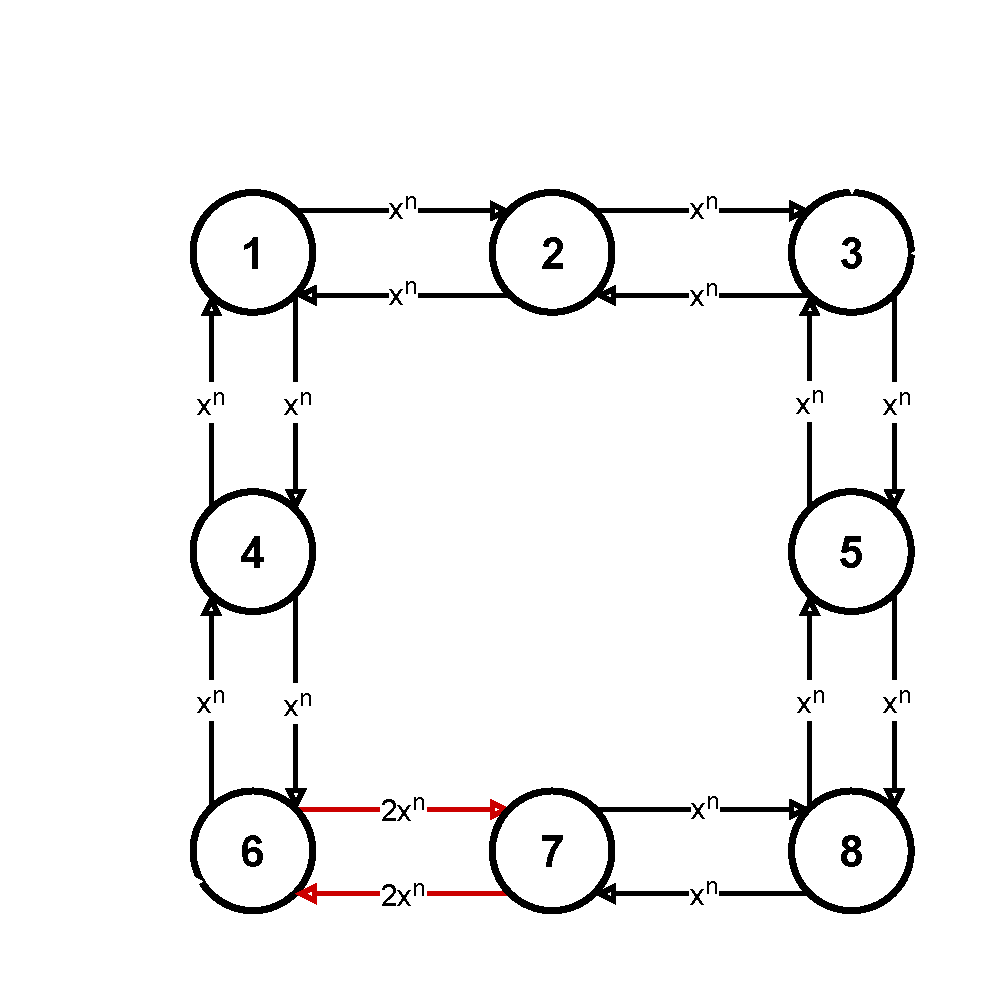
\includegraphics[width=\linewidth]{Img/cex_init.pdf}
    \end{minipage}
    \begin{minipage}{0.3\textwidth}
        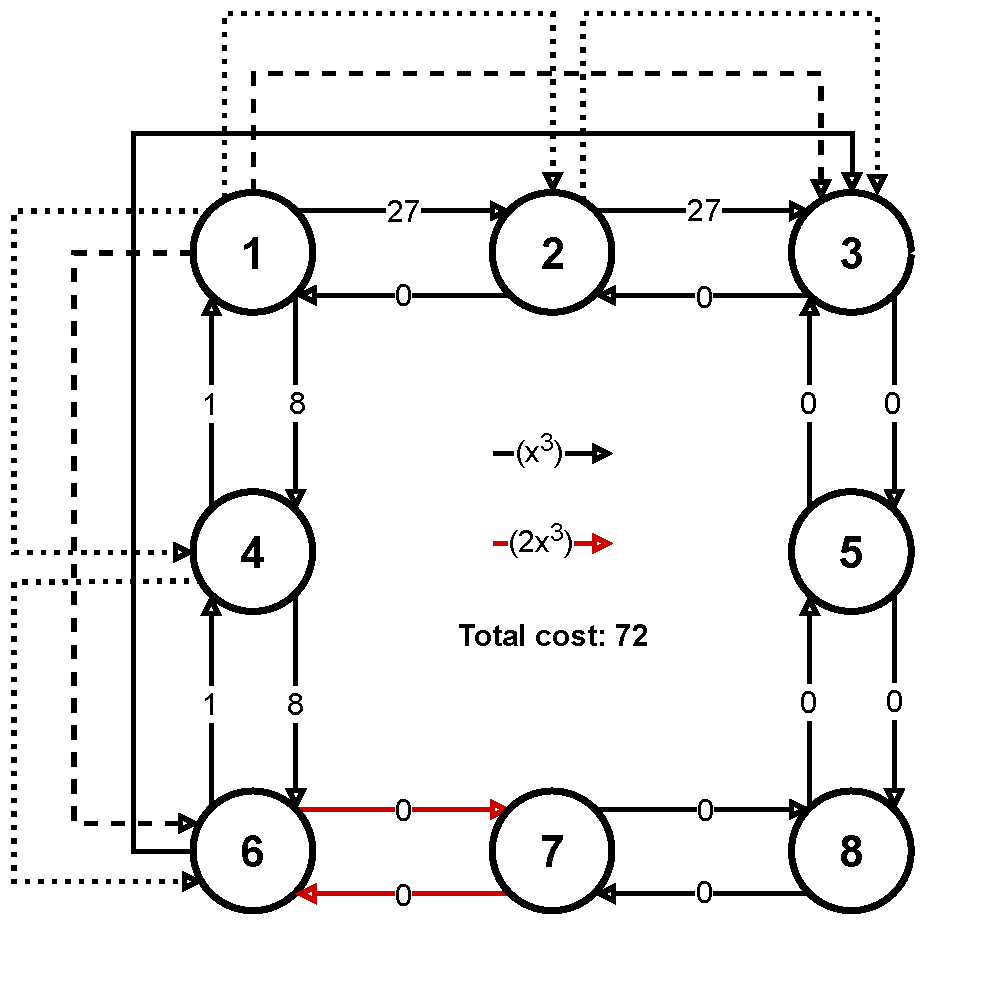
\includegraphics[width=\linewidth]{Img/cex_greedy.pdf}
    \end{minipage}
    \begin{minipage}{0.3\textwidth}
        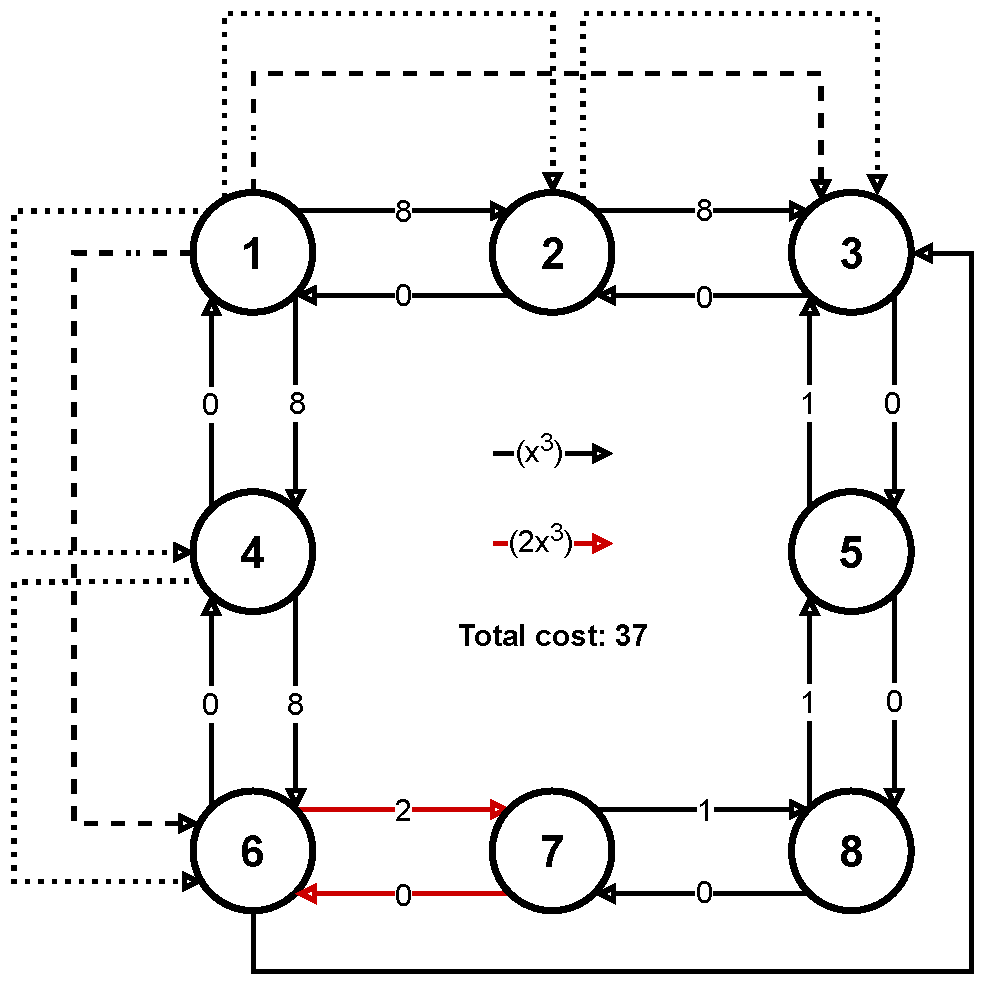
\includegraphics[width=\linewidth]{Img/cex_opt.pdf}
    \end{minipage}
    \captionof{figure}{Instance $4$, its MWU solution, and its optimal solution}
    \label{fig:cex}
}

\begin{figure}[!ht]
    \centering
    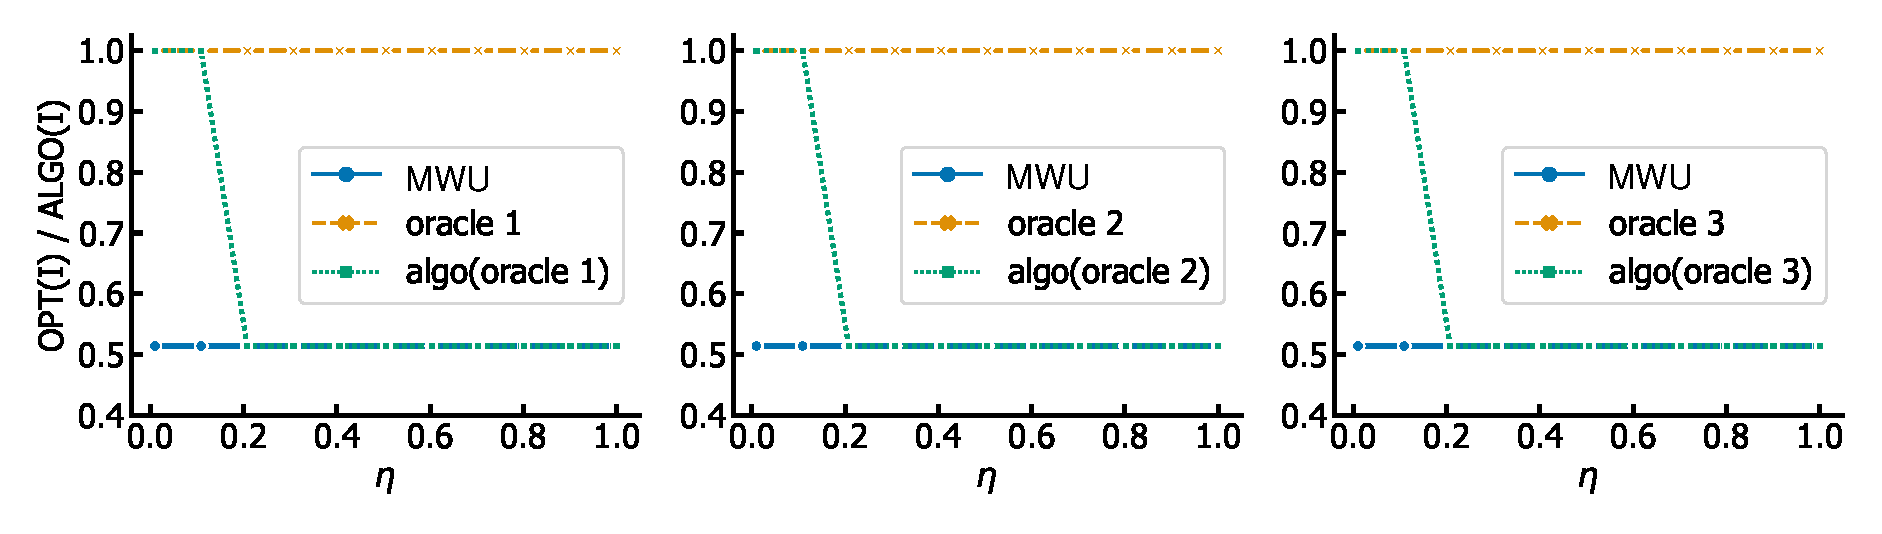
\includegraphics[width=\linewidth]{Img/cex_tight.pdf}
    \caption{Performance analysis of Instance $4$}
    \label{fig:cex-perf}
\end{figure}


\begin{figure}[!ht]
    \centering
    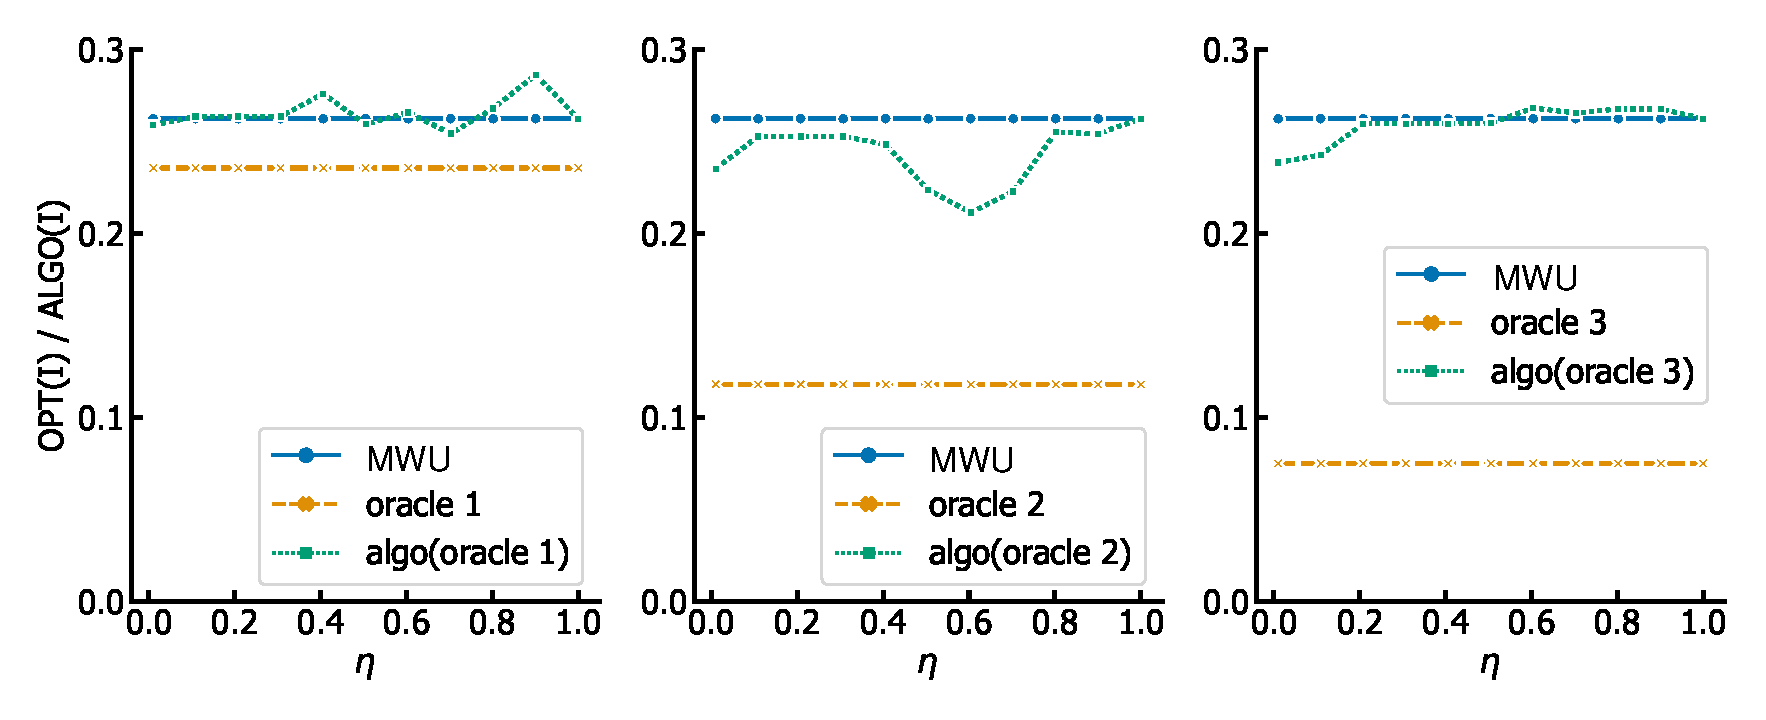
\includegraphics[width=\linewidth]{Img/random_tight.pdf}
    \caption{Performance analysis of Instance $1$}
    \label{fig:random}
\end{figure}


\begin{figure}[!ht]
    \centering
    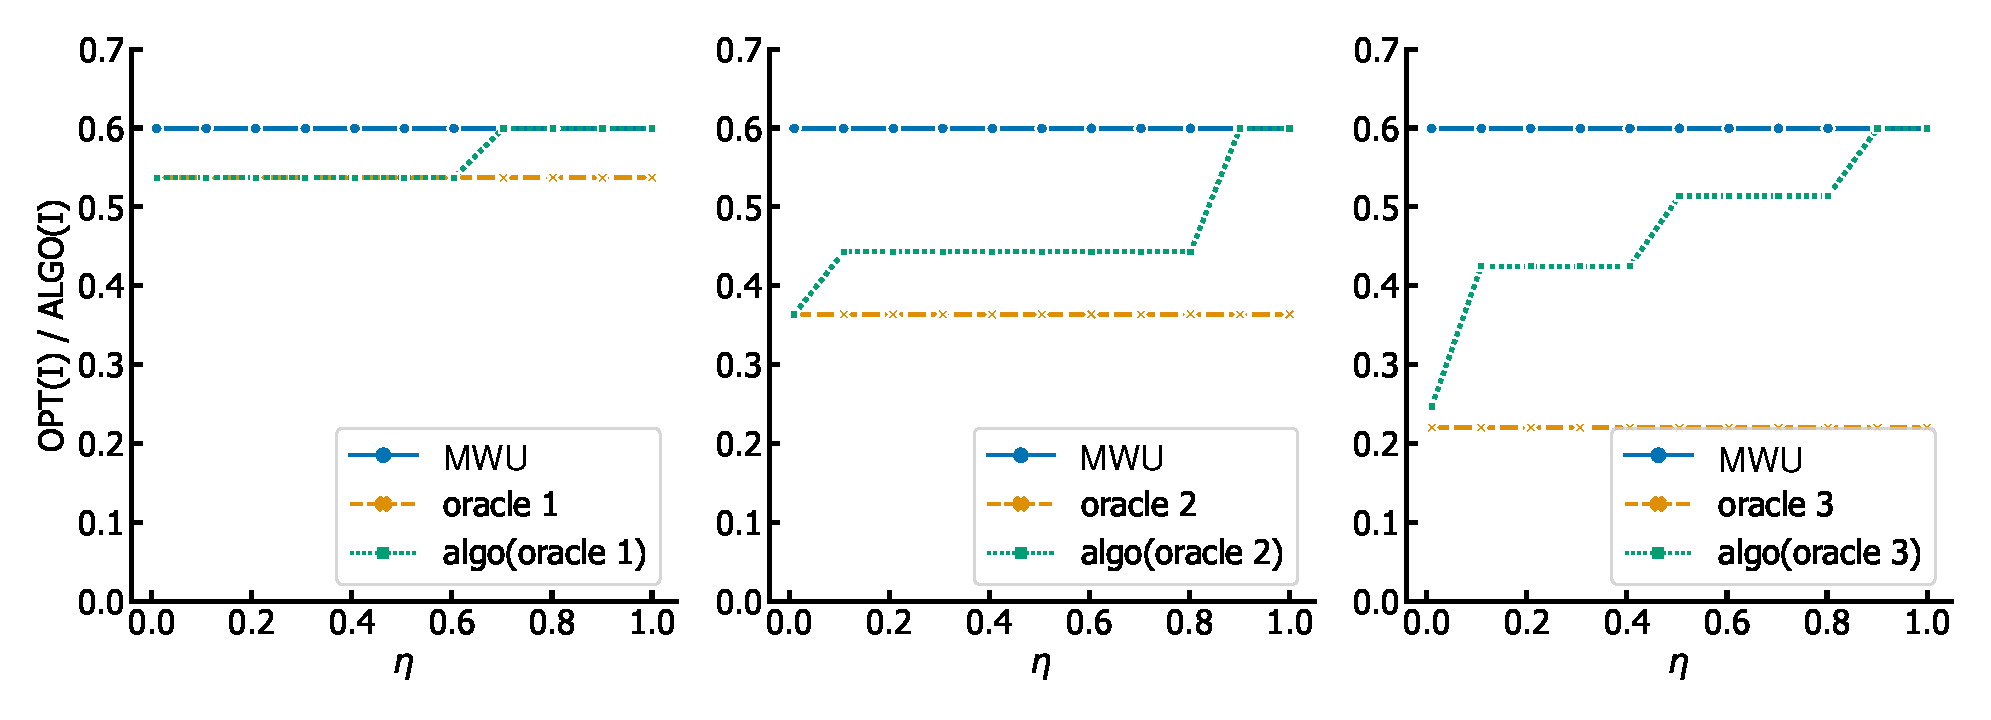
\includegraphics[width=\linewidth]{Img/random_small_tight.pdf}
    \caption{Performance analysis of Instance $2$}
    \label{fig:small-random}
\end{figure}

\begin{figure}[!ht]
    \centering
    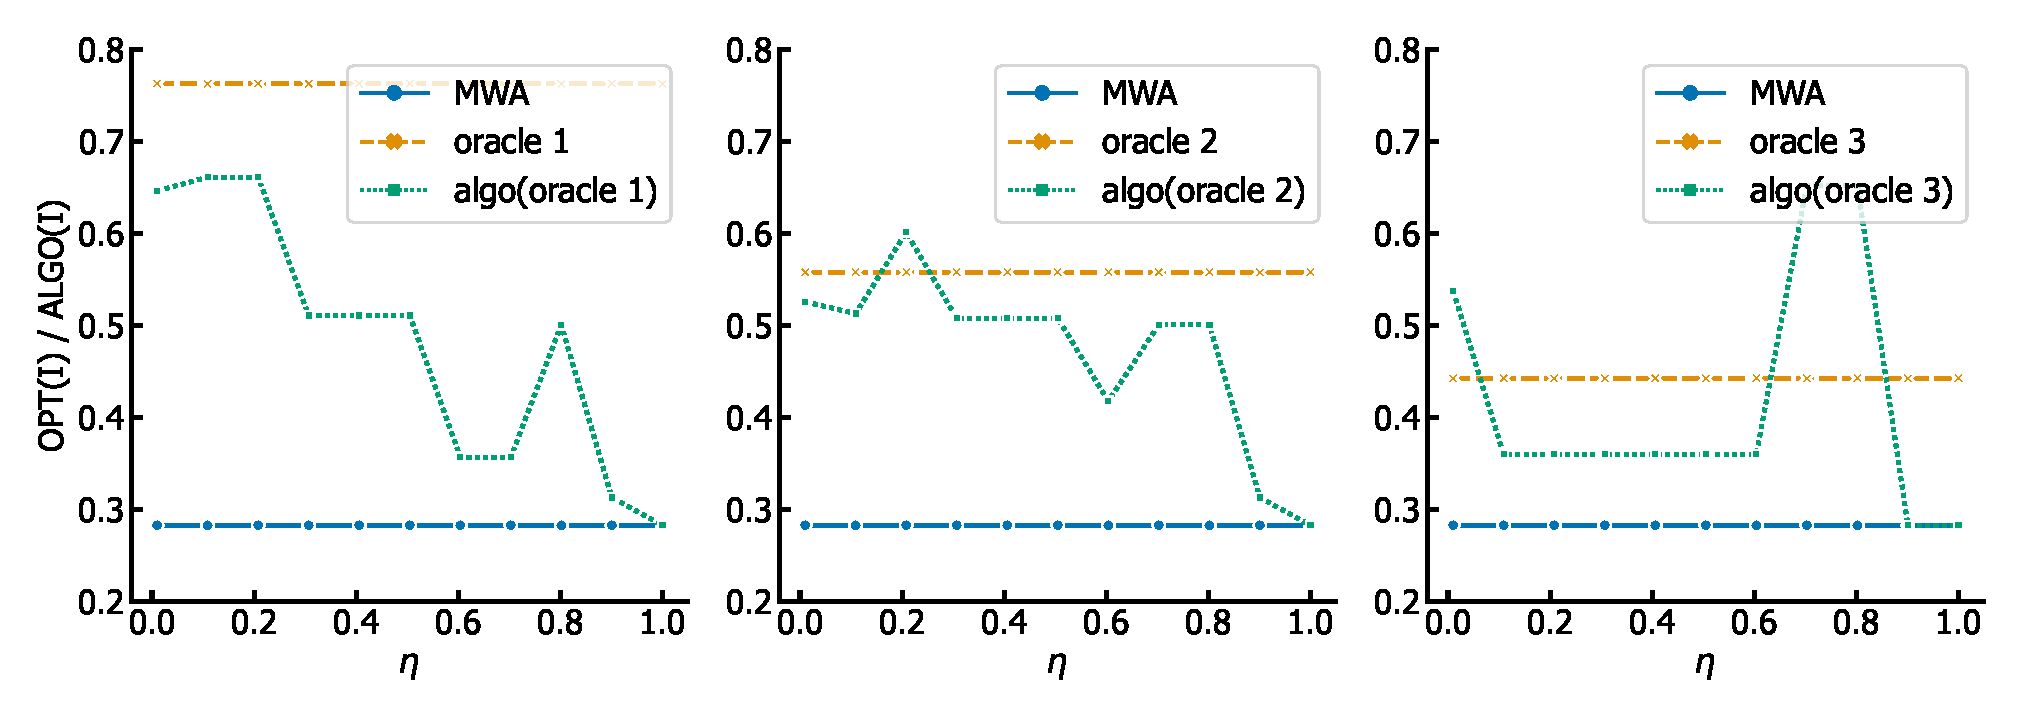
\includegraphics[width=\linewidth]{Img/connected_tight.pdf}
    \caption{Performance analysis of Instance $3$}
    \label{fig:connected}
\end{figure}

%!TEX root = ./main.tex

\section{Conclusion}

We presented a primal-dual framework to design algorithms with predictions for non-linear problems with covering constraints.
The potential of our approach is visible through the example applications, therefore this paper provides useful ideas to incorporate predictions into algorithms.
Our framework is of interest for many high impact applications, such as norm minimization, mixed packing and covering problems, energy minimization, and submodular minimization.

In our paper we answer two open questions.
First, we answer the question of \cite{BamasMaggiori20:The-Primal-Dual-method} to create a primal-dual framework for general problems with \emph{non-linear} objective functions and covering constraints.
Second, our work implies an \emph{optimal} competitive ratio of $O\bigl( k \cdot \log (d)\bigr)$ for the standard (without predictions) online problem of minimizing $\|C \vect{x}\|_{k}$ under covering constraints, answering an open question in \cite{NagarajanShen17:Online-Covering}. As a corollary, our algorithm provides an $O\bigl( \log m \cdot \log d \bigr)$-competitive solution to the online mixed packing and covering problem that is \emph{optimal} up to a constant factor.

An interesting research direction is to design algorithms for non-linear packing problems and also to develop competitive algorithms in the setting of multiple predictions.



\bibliography{references}

\appendix

%!TEX root = ./main.tex

\section*{Appendix}

\section{An example from the introduction} \label{apix:example-introduction}

The following example demonstrates why an approach where we alternate between the solutions of the prediction oracle and the primal-dual method does not work for non-linear objective functions.

Let us consider the objective of $x_{11}^p + ... + x_{1k}^p + x_{21}^p + ... + x_{2k}^p$ where $k$ and $p$ are some integers; and two algorithms: Algorithm $1$ and Algorithm $2$. At time $t$, the constraint is $x_{1t} + x_{2t} \geq 1$ and Algorithm $1$ always sets $x_{1t} = 1$ and Algorithm $2$ always sets $x_{2t} = 1$. Any alternating strategy has a cost of $1$ at any time $t$. The optimal cost is $1/2^p$ at any time $t$ by setting $x_{1t} = x_{2t} = 1/2$. The competitive ratio is $2^p$. We can generalize this example for $n$ algorithms ($n$ types of variables $x_{1t}, x_{2t}, ..., x_{nt}$). The same computation gives the competitive ratio of $n^p$. This ratio is not captured by any function intrinsically depending only on $\lambda$ and $\mu$ (as there is a parameter $n$ in the competitive ratio).

\section{Complete proof of \cref{lem:bound-x} in \cref{sec:covering}} \label{apix:lemma-proof}
\setcounter{theorem}{3}
\begin{restatable}{lemma}{BoundX}
	Let $e$ be an arbitrary resource.
	At any moment $\tau$ during the execution of the algorithm,
	when $t$ constraints have already been released, it always holds that
	$$
	x_{e}	\geq  \frac{\eta}{b^{t_{e}^{*}}_{e}(A) \ d}
			\left[ \exp\biggl( \frac{\ln(1+2d^{2}/\eta)}{\beta_{e}}
					\cdot \sum_{A: e \notin A} \sum_{t' \le t} b^{t'}_{e}(A) \cdot \alpha^{t'}_{A} \biggr) - 1 \right]
	$$
	where $b^{t_{e}^{*}}_{e}(A)$ is defined in the algorithm on line~\ref{algo-covering:bmax}.
\end{restatable}
\begin{proof}
	Let us fix a resource $e$ and prove the lemma by induction. At the beginning of the execution, when no constraint has been released yet, both sides of the lemma are 0.
	Let us assume that the lemma holds until the release of the $t^{\text{th}}$ constraint $\sum_{e} a^{t}_{e} x_{e} \geq 1$.
	Consider a moment $\tau$ during the algorithm's execution
	and let $A^{*}$ be the current set of resources $e'$ such that $x_{e'} = 1$.
	If at time~$\tau$, $x_{e} = 1$, then by the algorithm's design, the set $A^{*}$ has been updated such that
	$e \in A^{*}$. As such, the increasing rates of both sides in the lemma inequality are 0.
	In the remaining of the proof, we assume that  $x_{e} < 1$.
	We recall that by the algorithm's design, $\beta_{e} \geq \frac{1}{\lambda} \nabla_{e} F(\vect{x})$.
	We consider two cases $\beta_{e} > \frac{1}{\lambda} \nabla_{e} F(\vect{x})$
	and $\beta_{e} = \frac{1}{\lambda} \nabla_{e} F(\vect{x})$.

	\textbf{Case 1: $\beta_{e} > \frac{1}{\lambda} \nabla_{e} F(\vect{x})$.}
	In this case, by the algorithm's design, the value of $\beta_{e}$ remains unchanged at time~$\tau$ (line \ref{algo-covering:beta}) ($\frac{\partial \beta_{e}}{\partial \tau} = 0$).
	The lemma's right-hand side's derivative according to $\tau$ is
	\begin{align*}
	&\sum_{t' \le t} \frac{\partial \alpha^{t'}_{A^{*}}}{\partial \tau} \cdot
		\frac{b^{t'}_{e}(A^{*}) \ \eta }{b^{t_{e}^{*}}_{e}(A) \ d} \cdot \frac{\ln(1+2d^{2}/\eta)}{\beta_{e}}
			\cdot \exp\biggl( \frac{\ln(1+2d^{2}/\eta)}{\beta_{e} } \cdot \sum_{A: e \notin A} \sum_{t' \le t} b^{t'}_{e}(A)\ \alpha^{t'}_{A} \biggr) \\
	%
	&\leq \frac{\partial \alpha^{t}_{A^{*}}}{\partial \tau} \cdot
		\frac{b^{t}_{e}(A^{*}) \ \eta }{b^{t_{e}^{*}}_{e}(A) \ d} \cdot \frac{\ln(1+2d^{2}/\eta)}{\beta_{e}} \cdot \left( \frac{b^{t_{e}^{*}}_{e}(A) \ d}{\eta}\ x_{e} + 1 \right) \\
	%
	&= \frac{1}{\lambda \ln(1+2d^{2}/\eta)} \cdot
		\frac{b^{t}_{e}(A^{*}) \ \eta }{b^{t_{e}^{*}}_{e}(A) \ d} \cdot \frac{\ln(1+2d^{2}/\eta)}{\beta_{e}} \cdot \left( \frac{b^{t_{e}^{*}}_{e}(A) \ d}{\eta}\ x_{e} + 1 \right) \\
	%
	&\leq  \frac{b^{t}_{e}(A^{*}) \ x_{e}}{\lambda\ \beta_{e}} + \frac{\eta}{\lambda\ \beta_{e}\ d} \\
	%
	&\leq \frac{\partial x_{e}}{\partial \tau}
	\end{align*}
	%
	In the first inequality, we use the induction hypothesis and $\frac{\partial \alpha^{t}_{A^{*}}}{\partial \tau} > 0$
	and $\frac{\partial \alpha^{t'}_{A^{*}}}{\partial \tau} \leq 0$ for $t' < t$ and $\frac{\partial \beta_{e}}{\partial \tau} = 0$.
	The equality follows the increasing rate of $\alpha^{t}_{A^{*}}$.
	The last inequality is due to the increasing rate of $x_{e}$.
	The rate on the left-hand side is always larger than on the right-hand side, so the lemma inequality holds.

	\textbf{Case 2: $\beta_{e} = \frac{1}{\lambda} \nabla_{e} F(\vect{x})$.}
	In this case, by the algorithm's design, $\frac{1}{\lambda} \nabla_{e} F(\vect{x})$ is locally non-decreasing at $\tau$ (since otherwise,
	by line \ref{algo-covering:beta}, $\beta_{e}$ is not maintained to be equal to $\frac{1}{\lambda} \nabla_{e} F(\vect{x})$).
	Therefore, $\frac{\partial \beta_{e}}{\partial \tau} \geq 0$ and so $\partial \bigl(\frac{1}{\beta_{e}}\bigr)/\partial \tau \leq 0$.
	Hence, the derivative of the right-hand side of the lemma inequality according to $\tau$ is upper bounded by
	\begin{align*}
	\sum_{t' \le t} \frac{\partial \alpha^{t}_{A^{*}}}{\partial \tau} \cdot
		\frac{b^{t'}_{e}(A^{*}) \ \eta}{b^{t_{e}^{*}}_{e}(A) \ d} \cdot \frac{\ln(1+2d^{2}/\eta)}{\beta_{e}}
			\cdot \exp\biggl( \frac{\ln(1+2d^{2}/\eta)}{\beta_{e} } \cdot \sum_{A: e \notin A} \sum_{t' \le t} b^{t'}_{e}(A)\ \alpha^{t'}_{A} \biggr)
	\end{align*}
	which is bounded by $\frac{\partial x_{e}}{\partial \tau}$ by the same argument as the previous case. The lemma follows.
\end{proof}


\section{Complete proofs from application related propositions} \label{sec:appix-proofs}
To apply Theorem \ref{thm:covering-formal} on specific problems, we need to determine the local-smoothness parameters for the multilinear extension.
\cite{Thang20:Online-Primal-Dual} provided these parameters for some broad classes of functions, in particular for polynomials with non-negative coefficients. Let $g_{\ell}: \mathbb{R} \rightarrow \mathbb{R}$ for $1 \leq \ell \leq L$
be degree-$k$ polynomials with non-negative coefficients and let $f:~\{0,1\}^{n}~\rightarrow~\mathbb{R}^{+}$ be the cost function
defined as $f(\one_{S}) = \sum_{\ell} b_{\ell} g_{\ell}\bigl( \sum_{e \in S} a_{e} \bigr)$ where $a_{e} \geq 0$ for every
$e$ and $b_{\ell} \geq 0$ for every $1 \leq \ell \leq L$.
Then the multilinear extension $F$ of $f$ is $(O(k \ln(d/\eta))^{k-1}, \frac{k-1}{k \ln(1 + 2d^{2}/\eta)})$-locally smooth.
We will use these parameters to derive the guarantees for the following problems.


%%% **************************
%%% **************************
%%% **************************

\subsection{Energy Minimization in Scheduling}

Reducing carbon emissions is a global effort in which energy-efficient algorithms play an essential role. For example, \cite{Albers10:Energy-efficient-algorithms} and \cite{GuCaiZengZhangJinDai:2019} studied energy-efficient algorithms for scheduling.

Given $m$ unrelated machines, we need to assign jobs that arrive online. Each job $j$ has a release date $r_{j}$, a deadline $d_{j}$, and a vector of machine dependent processing times $p_{ij}$. Contrary to performance-oriented scheduling, our goal is to design an assignment policy which can minimize the total energy consumption of the execution. To achieve this, we can adjust the machines' speed $s_{ij}(t)$ during the time interval $[t,t+1)$ for the execution of job $j$. Every machine $i$ has a non-decreasing energy power function $P_{i}(\cdot)$. Typically, $P_{i}(z) = z^{k_{i}}$ for some constant $k_{i} \geq 1$. The execution's total energy is $\sum_{i} \sum_{t} P(\sum_{j} s_{ij}(t))$.

In the classic online setting, this problem is well understood: there exists an $O(k^{k})$-competitive algorithm \cite{Thang20:Online-Primal-Dual} where $k = \max_{i} \{k_{i}\}$
and this bound is tight up to a constant factor \cite{Caragiannis08:Better-bounds}. In our extended study with predictions we represent this problem with the following non-linear program. The objective is $\min \sum_{i} \sum_{t} P(\sum_{j} s_{ij}(t))$ and the constraints are:
$$
\sum_{i=1}^{m} x_{ij} = 1,  \qquad \qquad \sum_{t = r_{j}}^{d_{j}-1} s_{ij}(t) \geq p_{ij} x_{ij}, \qquad  \qquad s_{ij}(t) \geq 0  \qquad \forall\ i,\ t
$$
where $x_{ij} \in \{0,1\}$ indicates whether job $j$ is assigned to machine $i$
and $s_{ij}(t) \geq 0$ denotes the speed of machine $i$ executing job $j$ during the time interval $[t, t+1)$.
The first constraint guarantees that job $j$ is assigned to some machine, and the second one ensures
that the job $j$ is completed on time (on the machine where the job is assigned). At the arrival of
job $j$, the prediction provides a solution $pred(x_{ij})$ and a speed $pred(s_{ij}(t))$ for $r_{j} \leq t \leq d_{j} - 1$.
Using our framework, we can deduce the following result.

\setcounter{theorem}{7}
\begin{proposition}
Algorithm~\ref{algo:covering} gives a
$O(\frac{1}{1 - \eta})$-consistent and $O\bigl(k^{k} \log^{k} \frac{m}{\eta}\bigr)$-robust fractional solution
for the energy minimization problem.
\end{proposition}
%
\begin{proof}
The objective function $\sum_{i} \sum_{t} P(\sum_{j} s_{ij}(t))$ is a polynomial of degree $k = \max_{i} k_{i}$;
so its multilinear extension is
$(O(k \ln(m/\eta))^{k-1}, \frac{k-1}{k \ln(1 + 2m^{2}/\eta)})$-locally smooth
(the maximal number of positive coefficients in a constraint $d = m$).
Therefore, applying Theorem~\ref{thm:covering-formal},
Algorithm~\ref{algo:covering} provides a $O(\frac{1}{1 - \eta})$-consistent and $O\bigl(k^{k} \ln^{k} \frac{m}{\eta}\bigr)$-robust
fractional solution.
\end{proof}



%%% **************************
%%% **************************
%%% **************************

\subsection{Online Submodular Mimimization}	\label{apix:sub-min}

Submodular minimization is a widespread subject in optimization and machine learning \cite{IwataFleischer01:A-combinatorial-strongly,Bachothers13:Learning-with,Bach16:Submodular-functions:,BalkanskiSinger:2020}. Let us consider the problem of minimizing an online monotone submodular function subject to covering constraints.
A set-function $f: 2^{\mathcal{E}} \rightarrow \mathbb{R}+$ is \emph{submodular} if
$f(S \cup e) - f(S) \geq f(T \cup e) - f(T)$ for all $S \subset T \subseteq \mathcal{E}$.
Let $F$ be the multilinear extension of a monotone submodular function $f$. Function $F$
admits two useful properties. First, if $f$ is monotone, then so is $F$. Second, $F$ is concave in
the positive direction, meaning that $\nabla F(\vect{x}) \geq \nabla F(\vect{y})$ for all $\vect{x} \leq \vect{y}$, where $\vect{x} \leq \vect{y}$ is defined as $x_{e} \leq y_{e} ~\forall e$.

To apply Algorithm~\ref{algo:covering}, we need to determine the local-smoothness parameters.
An important concept in studying submodular functions is the \emph{curvature}. Given a submodular
function $f$, the \emph{total curvature} $\kappa_{f}$ (\cite{ConfortiCornuejols84:Submodular-set-functions}) of $f$ is defined as
$
\kappa_{f} = 1 - \min_{e} \frac{f(\one_{\mathcal{E}}) - f(\one_{\mathcal{E} \setminus \{e\}})}{f(\one_{\{e\}})}.
$
Intuitively, the total curvature measures how far away $f$ is from being \emph{modular}. This concept of
curvature is used to determine both upper and lower bounds on the approximation ratios
for many submodular and learning problems (see \cite{ConfortiCornuejols84:Submodular-set-functions,GoemansHarvey09:Approximating-submodular,BalcanHarvey12:Learning-Submodular,Vondrak10:Submodularity-and-Curvature:,IyerJegelka13:Curvature-and-optimal,SviridenkoVondrak17:Optimal-approximation}).
The following lemma shows a useful property of the total curvature.

\setcounter{theorem}{8}
\begin{proposition}
Algorithm~\ref{algo:covering} gives a
$O(\frac{1}{1 - \eta})$-consistent and $O\bigl( \frac{\log (d/\eta)}{1 - \kappa_{f}} \bigr)$-robust fractional  solution
for the submodular minimization under covering constraints.
\end{proposition}
\begin{proof}
Let $F$ be the multilinear extension of $f$.
It is sufficient to verify that $F$ is $\bigl(\frac{1}{1-\kappa_{f}},0\bigr)$-locally smooth.
Recall that, by definition of the multilinear extension,
$F(\vect{x}) = \mathbb{E} \bigl[ f(\one_{T})\bigr]$ where $T$ is a random set
such that a resource $e$ appears in $T$ with probability $x_{e}$. Moreover, as $F$ is linear in $x_{e}$, we have
%
\begin{align*}
\nabla_{e} F(\vect{x}) %= \frac{\partial F(\vect{x}) }{\partial x_{e}}
&= F(x_{1}, \ldots, x_{e-1}, 1, x_{e+1}, \ldots, x_{n}) - F(x_{1}, \ldots, x_{e-1}, 0, x_{e+1}, \ldots, x_{n}) \\
&= \mathbb{E} \biggl[ f\bigl(\one_{R \cup \{e\}}\bigr) - f\bigl(\one_{R}\bigr) \biggr]
\end{align*}
where $R$ is a random subset of resources $N \setminus \{e\}$ such that $e'$ is included with probability $x_{e'}$.
Therefore, to prove that $F$ is $(\lambda,\mu)$-locally-smooth, it is equivalent to show that,
for any set $S \subset \mathcal{E}$ and for any vectors $\vect{x}^{e} \in [0,1]^{n}$ for $e \in \mathcal{E}$,
%
\begin{equation*}	\label{eq:min-local-smooth-equiv}
\sum_{e \in S} \mathbb{E} \biggl[ f\bigl(\one_{R^{e} \cup \{e\}}\bigr) - f\bigl(\one_{R^{e}}\bigr) \biggr]
\leq \lambda f\bigl( \one_{S} \bigr) + \mu \mathbb{E} \biggl[ f\bigl(\one_{R}\bigr) \biggr]
\end{equation*}
%
where $R^{e}$ is a random subset of resources $N \setminus \{e\}$ such that $e'$ is included with probability $x^{e}_{e'}$
and $R$ is a random subset of resources $N \setminus \{e\}$ such that $e'$ is included with probability $\max_{e \in S} x^{e}_{e'}$.

The $\bigl(\frac{1}{1-\kappa_{f}},0\bigr)$-local smoothness of $F$ holds due to submodularity and \cref{lem:curvature} (see below), so
for any subsets $R^{e}$, we have
\begin{align*}
	\sum_{e \in S} \left[ f\bigl(\one_{R^{e} \cup \{e\}}\bigr) - f\bigl(\one_{R^{e}}\bigr) \right]
		\leq \sum_{e \in S} \left[ f\bigl(\one_{\{e\}}\bigr) \right]
		\leq \frac{1}{1 -\kappa_{f}} \cdot f(\one_{S})
\end{align*}
Therefore, applying Theorem~\ref{thm:covering-formal}, the proposition follows.
%Algorithm~\ref{algo:covering} gives a fractional
%$O(\frac{1}{1 - \eta})$-consistent and $O\bigl( \frac{\log (d/\eta)}{1 - \kappa_{f}} \bigr)$-robust solution.
\end{proof}

\begin{lemma}		\label{lem:curvature}
	For any set $S$, it always holds that
	$$
	f(\one_{S}) \geq (1-\kappa_{f}) \sum_{e \in S} f(\one_{\{e\}}).
	$$
\end{lemma}
\begin{proof}
	Let $S = \{e_{1}, \ldots, e_{m}\}$ be an
	arbitrary subset of $\mathcal{E}$. Let $S_{i} = \{e_{1}, \ldots, e_{i}\}$ for $1 \leq i \leq m$ and $S_{0} = \emptyset$.
	We have
	\begin{align*}
	f(\one_{S})
	&\geq  f(\one_{\mathcal{E}}) -  f(\one_{\mathcal{E} \setminus S})
	= \sum_{i=0}^{m-1}  f(\one_{\mathcal{E} \setminus S_{i}}) - f(\one_{\mathcal{E} \setminus S_{i+1}})
	\geq \sum_{i=1}^{m}  f(\one_{\mathcal{E}}) - f(\one_{\mathcal{E} \setminus \{e_{i}\}}) \\
	&\geq (1 - \kappa_{f}) \sum_{i=1}^{m} f(\one_{e_{i}})
	\end{align*}
	where the first two inequalities are due to the submodularity of $f$, and the last inequality follows the definition of curvature.
\end{proof}


\end{document}
